\documentclass[kpfonts,lotsofwhite]{patmorin}
\usepackage[UKenglish]{babel}
\usepackage[T1]{fontenc}
 % Something in here is breaking cleveref
 %\usepackage{lmodern,amsmath,amsthm,amsfonts,amssymb,graphicx,float,microtype,thmtools,underscore,mathtools}
 \usepackage{graphicx,amsmath,amsthm,amsfonts,amssymb,mathtools}
% \usepackage[shortlabels]{enumitem}
% \setlist[itemize]{topsep=0ex,itemsep=0ex,parsep=0ex}
% \setlist[enumerate]{topsep=0ex,itemsep=0ex,parsep=0ex}
\usepackage[usenames,dvipsnames,svgnames,table]{xcolor}
%%%%
%\usepackage{breakurl} %needed for arXiv
% \usepackage[unicode=true]{hyperref}
% \hypersetup{
% 	colorlinks,
% 	linkcolor={blue!60!black},
% 	citecolor={black},
% 	urlcolor={blue!60!black},
% 	pdftitle={Grid Minors and Products}}
%%%
\usepackage[capitalise, compress, nameinlink, noabbrev]{cleveref}
\usepackage{cleveref}
\crefname{lem}{Lemma}{Lemmas}
\crefname{thm}{Theorem}{Theorems}
\crefname{cor}{Corollary}{Corollaries}
%%%
\newcommand{\defn}[1]{\textcolor{Maroon}{\emph{#1}}}
\newcommand{\mathdefn}[1]{\textcolor{Maroon}{#1}}
%%%%%%%%%%%%%%%%%%%%%%%%%%%%%%%%%%%%%%%%%%
\usepackage[longnamesfirst,numbers,sort&compress]{natbib}
% \makeatletter
% \def\NAT@spacechar{~}
% \makeatother
% \setlength{\bibsep}{0.4ex plus 0.2ex minus 0.2ex}
%%%%%%%%%%%%%%%%%%
% \usepackage[margin=28mm]{geometry}
% \renewcommand{\baselinestretch}{1.1}
% \setlength{\footnotesep}{\baselinestretch\footnotesep}
% \setlength{\parindent}{0cm}
% \setlength{\parskip}{1.2ex}
% \allowdisplaybreaks
%%%%%%%%%%
\usepackage{todonotes}
\graphicspath{{figs/}}
\usepackage{paralist}
\newcommand{\boxprod}{\mathbin{\Box}}
\newcommand{\N}{\mathbb{N}}
%%%%
\newcommand{\half}{\ensuremath{\protect\tfrac{1}{2}}}
\DeclarePairedDelimiter{\floor}{\lfloor}{\rfloor}
\DeclarePairedDelimiter{\ceil}{\lceil}{\rceil}
\DeclarePairedDelimiter{\abs}{\lvert}{\rvert}
\DeclarePairedDelimiter{\set}{\{}{\}}
%%%% Commands
\renewcommand{\epsilon}{\varepsilon}
\renewcommand{\emptyset}{\varnothing}
\renewcommand{\ge}{\geqslant}
\renewcommand{\le}{\leqslant}
\renewcommand{\geq}{\geqslant}
\renewcommand{\leq}{\leqslant}
%%%
\DeclareMathOperator{\polylog}{polylog}
\DeclareMathOperator{\wcol}{wcol}
\DeclareMathOperator{\col}{col}
\DeclareMathOperator{\dist}{dist}
\DeclareMathOperator{\tw}{tw}
\DeclareMathOperator{\gm}{gm}
\DeclareMathOperator{\tpw}{tpw}
\DeclareMathOperator{\pw}{pw}
\DeclareMathOperator{\td}{td}
\DeclareMathOperator{\sep}{sep}
\DeclareMathOperator{\stw}{stw}
\DeclareMathOperator{\ltw}{ltw}
\DeclareMathOperator{\rtw}{rtw}
%%
\newcommand{\RR}{\mathbb{R}}
\newcommand{\JJ}{\mathcal{J}}
\newcommand{\PP}{\mathcal{P}}
\newcommand{\BB}{\mathcal{B}}
\newcommand{\FF}{\mathcal{F}}
\newcommand{\GG}{\mathcal{G}}
\newcommand{\HH}{\mathcal{H}}
\newcommand{\LL}{\mathcal{L}}
\newcommand{\NN}{\mathbb{N}}
\newcommand{\OO}{\mathcal{O}}
\newcommand{\WW}{\mathcal{W}}
\newcommand{\scr}[1]{\mathcal{#1}}
\newcommand{\ds}[1]{\mathbb{#1}}
%%%
\newcommand{\david}[1]{{\color{orange} DW: #1}}
\newcommand{\vida}[1]{{\color{DarkGreen} V: #1}}
\newcommand{\pat}[1]{\textcolor{Maroon}{PM: #1}}

\newcommand{\worley}[1]{\textcolor{Purple}{DAW: #1}}
%%%
% \renewcommand{\thefootnote}{\fnsymbol{footnote}}
%%%
\theoremstyle{plain}
\newtheorem{thm}{Theorem}
\newtheorem{lem}[thm]{Lemma}
\newtheorem{cor}[thm]{Corollary}
\newtheorem{ques}[thm]{Question}
\newtheorem{prop}[thm]{Proposition}
\newtheorem{obs}[thm]{Observation}
\newtheorem*{claim}{Claim}
\crefname{obs}{Observation}{Observations}
\newtheorem*{lem*}{Lemma}
\theoremstyle{definition}
\newtheorem{conj}[thm]{Conjecture}
\newtheorem*{conj*}{Conjecture}
%%%%%%%%%%%%%%%%%%%%%%%%%%%%%%%%%%%%%%%%%%%%%%

\begin{document}
\title{\bf\boldmath\fontsize{18pt}{18pt}\selectfont
Grid Minors and Products}

\author{
Vida Dujmovi{\'c}\,\footnotemark[3]\qquad
Pat Morin\,\footnotemark[4]\qquad
David~R.~Wood\,\footnotemark[2]\qquad
and David~Worley\footnotemark[5]
}

\maketitle

\begin{abstract}
    We show that the Cartesian product of any two connected $n$-vertex graphs contains an $\Omega(\sqrt{n})\times\Omega(\sqrt{n})$ grid minor.  This result is tight: The product of an $n$-vertex star and an $n$-vertex path has no $\omega(\sqrt{n})\times\omega(\sqrt{n})$ grid minor.
\end{abstract}

\footnotetext[2]{School of Mathematics, Monash University, Melbourne, Australia (\texttt{david.wood@monash.edu}). Research supported by the Australian Research Council. }

%\footnotetext[2]{School of Mathematics, Monash University, Melbourne, Australia (\texttt{\{marc.distel,robert.hickingbotham, david.wood\}@monash.edu}). Research of Wood supported by the Australian Research Council. Research of Distel and Hickingbotham supported by Australian Government Research Training Program Scholarships.}

\footnotetext[3]{School of Computer Science and Electrical Engineering, University of Ottawa, Ottawa, Canada (\texttt{vida.dujmovic@uottawa.ca}). Research supported by NSERC.}

%\footnotetext[3]{Computer Science Department, University of California, Irvine (\texttt{eppstein@uci.edu}). Research supported in part by NSF grant CCF-2212129.}

%\footnotetext[4]{D\'epartement d'Informatique, Universit\'e Libre de Bruxelles, Belgium (\texttt{gwenael.joret@ulb.be}). Supported by an ARC grant from the Wallonia-Brussels Federation of Belgium and a CDR grant from the National Fund for Scientific Research (FNRS).}

%\footnotetext[5]{Department of Theoretical Computer Science, Jagiellonian University, Kraków, Poland (\texttt{michal.seweryn@tcs.uj.edu.pl}).}

\footnotetext[4]{School of Computer Science, Carleton University, Ottawa, Canada (\texttt{morin@scs.carleton.ca}). Research supported by NSERC.}

\footnotetext[5]{School of Computer Science and Electrical Engineering, University of Ottawa, Ottawa, Canada (\texttt{dworl020@uottawa.ca}). Research supported by NSERC.}

%\newpage
%\section{\Large Introduction}


\section{Introduction}

The current research is motivated by two recent developments. The first is the use of graph product structure theory to resolve a number of longstanding open problems on planar graphs and their relatives.  The second is the role of strong excluded grid minor theorems in approximation algorithms for NP-hard problems on planar and related graph classes.  We now elaborate on both these topics.

TODO: Define graph products $\boxprod$ and $\boxtimes$ and explain the planar product structure theorem.

TODO: Define the subquadratic grid minor property and the state-of-the art in excluded grid minors.
For every positive integer $k$, let $\boxplus_k$ denote the $k\times k$ \defn{grid graph}, with vertex set $V(\boxplus_k):=[k]\times[k]$ and that contains an edge with endpoints $(x_1,y_1)$ and $(x_2,y_2)$ if and only $|x_1-x_2| + |y_1-y_2|=1$.\footnote{For every positive integer $k$, $[k]:=\{1,\ldots,k\}$.}  For a graph $G$, let $\tw(G)$ denote the treewidth\footnote{TODO: definition of treewidth} of $G$ and let $\gm(G)$ denote the largest integer $k$ such that $G$ contains a $\boxplus_k$ minor.\footnote{A graph $G_1$ is a \defn{minor} of a graph $G_2$ if a graph isomorphic to $G_1$ can be obtained from a subgraph of $G_2$ through a sequence of edge contractions.}

In this paper, we prove the following results:

\begin{enumerate}
   \item  For any two $n$-vertex connected graphs $G_1$ and $G_2$, $\gm(G_1\boxprod G_2) \in \Omega(\sqrt{n})$.
   \item There exists two $n$-vertex connected graphs $G_1$ and $G_2$ (a star and a path) such that $\gm(G_1\boxprod G_2) \in O(\sqrt{n})$.
\end{enumerate}

It is known that $\tw(G_1\boxprod G_2)\in\Theta(n)$ when $G_1$ and $G_2$ are $n$-vertex connected graphs.  Thus, the first result above gives an excluded grid theorem for graph products that is much stronger than the current best bound for general graphs. Indeed, the result of \cite{CT19} only implies that $\gm(G_1\boxprod G_2) \ge n^{1/9}/\log^{O(1)} n$.  Unfortunately, our results falls just short of being strong enough to allow the SQGM framework to be directly applied to graph products and the upper bound in the second result shows that this is by necessity.  TODO: Point to future work.

\section{Preliminaries}

In this paper, every graph $G$ is undirected and simple with vertex set $V(G)$ and edge set $E(G)$. The \defn{order} of $G$ is denoted $|G|:=|V(G)|$.
 See \citet{D10} for graph-theoretic definitions not given here.



% For any set $S$, the \defn{induced subgraph} $G[S]$ has $V(G[S]):=S\cap V(G)$ and $E(G[S]):=\{vw\in E(G):v,w\in S\}$. For any set $S$, $G-S = G[V(G)\setminus S]$.

For two graphs $G_1$ and $G_2$ we use the notation $G_1\preceq G_2$ to indicate that $G_1$ is a minor of $G_2$.  We make use of the fact that the $\preceq$ relation is transitive. The following observation follows immediately from definitions.

\begin{obs}\label{minor_product}
  Let $G_1$, $G_2$, and $H$ be graphs.  If $G_1\preceq G_2$, then $G_1\boxprod H\preceq G_2\boxprod H$.
\end{obs}

A \defn{model} of a graph $G_1$ in another graph $G_2$ is a set $\mathcal{M}:=\{B_x\subseteq V(G_2): x\in V(G_1)\}$ of subsets of $V(G_2)$, called \defn{branch sets}, indexed by the vertices of $G_1$ and such that
\begin{compactenum}[(i)]
  \item for each distinct pair $x,y\in V(G_1)$, $B_x\cap B_y=\emptyset$;
  \item for each $x\in V(G_1)$, $G_2[B_x]$ is connected and
  \item for each $xy\in E(G_1)$ there exists an edge $vw\in E(G_2)$ with $v\in B_x$ and $w\in B_y$.
\end{compactenum}
It follows from definitions that $G_1\preceq G_2$ if and only if there exists a model of $G_1$ in $G_2$.

For each $n\in N$, let $P_n$ denote an $n$-vertex path, and let $S_n$ denote the \defn{$n$-star}; the tree with $n$ leaves, each of which adjacent to the root.  For each $\ell,p\in\N$, let $S_{\ell,p}$ denote the star with $\ell$ leaves whose edges have been subdivided $p-1$ times.  More formally, $V(S_{\ell,p}):=\{v_0\}\cup\{v_{i,j}:(i,j)\in[\ell]\times[p]\}$ and $E(S_{\ell,p}):=\{v_0v_{i,1}:i\in[\ell]\}\cup \{v_{i,j}v_{i,j+1}:(i,j)\in[\ell]\times[p-1]\}$.  We call $S_{\ell,p}$ a \defn{subdivided star}.  Subdivided stars generalize both stars and paths: The $n$-vertex path $P_n$ is isomorphic to $S_{1,n-1}$ and the $n$-leaf star $S_n$ is isomorphic to $S_{n,1}$.

\begin{lem}\label{anything_times_star}
  For any positive integer $n$ and any $n$-vertex connected graph $G$, $K_{n} \preceq G\boxprod S_n$.
\end{lem}

\begin{proof}
  Let $y_0$ denote the root of $S_n$, let $y_1,\ldots,y_n$ denote the leaves of $S_n$.  We will show the existence of a model $\mathcal{M}:=\{B_x:x\in V(K_n)\}$ of $K_n$ in $G\boxprod S_n$.  Let $x_1,\ldots,x_{n}$ denote the vertices of $K_{n}$ and let $v_1,\ldots,v_n$ denote the vertices of $G$.  For each $i\in[n]$, define the branch set
  \[
     B_{x_i}:=\{(v,y_i):v\in V(G)\} \cup \{ (v_{i},y_0) \} \enspace .
  \]
  We now show that $\mathcal{M}$ is a model of $K_n$ in $G\boxprod S_n$.
  The induced graph $G[B_{v_i}]$ is connected because $G[\{(v,y_i):v\in V(G)\}]$ is isomorphic to $G$ and $(v_{i},y_0)$ is adjacent to $(v_{i},y_i)$.
  For any $1\le i< j\le n$, $B_{v_i}$ and $B_{v_j}$ are disjoint because $y_i\neq y_j$ and $v_i\neq v_j$.  Furthermore, the vertex $(v_{i},y_0)\in B_{x_i}$ is adjacent to $(v_i,y_j)\in B_{x_j}$.  Therefore, there is an edge in $G\boxprod S_n$ with one endpoint in $B_{v_i}$ and one endpoint of $B_{v_j}$ for each $1\le i < j\le n$.
\end{proof}

Note that, for any tree with $T$ with $n$ leaves and at least one non-leaf vertex, $S_n\preceq T$.  In this case, \cref{anything_times_star,minor_product} implies that $K_n\preceq G\boxprod T$.

\section{The Lower Bound}

% Our lower bound, which shows that, for any two $n$-vertex connected graphs $G_1$ and $G_2$, $\gm(G_1\boxprod G_2)\in\Omega(\sqrt{n})$ is obtained as follows:  We first show that each of $G_1$ and $G_2$ contains a `large' subdivided star.  Then we show that the product of any two `large' subdivided stars $S_{\ell_1, p_1}$ and $S_{\ell_2, p_2}$ contains a large grid-minor.  The quotes on `large' here are due to the fact that we measure the size of a subdivided star in a non-standard way, as in the following lemma.

\subsection{Connected Graphs Contain Large Subdivided Stars}

% We begin with a lemma which shows that every connected $n$-vertex graph contains a model of an $\Omega(n/\log n)$-vertex subdivided star.


% \textbf{Old Lemma and Proof}

% \begin{lem}\label{subdivided_star_minor}
% For every tree $T$ with $n\ge 2$ vertices, there exists integers $\ell,p$ with $\ell p\geq \frac{n-1}{2(\log (n-1)+1)^2}$, a subtree $R$ of $T$ and disjoint paths $P_1,\dots,P_\ell$ in $T-V(R)$, such that for each $i\in\{1,\dots,\ell\}$, one endpoint of $P_i$ is adjacent to some vertex in $R$, and $|V(P_i)|=p$.
% \end{lem}

% \begin{proof}
%   We make use of the \emph{heavy path decomposition} introduced by \citet{ST83} in the context of data structures.  Consider a tree $T$ rooted at a vertex $x$. For each vertex $v$, say a child $w$ of $v$ is \defn{heavy} if the subtree rooted at $w$ has at least as many vertices as each of the subtrees rooted at the other children of $v$. For each vertex $v_1$ of $T$, say a path $(v_1,\dots,v_k)$ in $T$ is \defn{heavy} if $v_{i+1}$ is a heavy child of $v_i$ for each $i\in\{1,\dots,k-1\}$, and $v_k$ is a leaf.

%   Let $\PP=\{P_1,\dots,P_m\}$ be the set of paths obtained from the following algorithm:

% initialise $i:=0$ and $P_0:=\{x\}$ \\
% while $V(T)\neq V(P_0\cup\dots\cup P_i)$ do\\
%  \hspace*{4mm}     increment $i$\\
% \hspace*{4mm} let $T_{i+1}$ be a component subtree of $T-V(P_1\cup\dots\cup P_i)$\\
% \hspace*{4mm} let $P_{i+1}$ be a heavy path in $T_{i+1}$ starting at the root of $T_{i+1}$\\
% end-while

%   Define the \defn{subtree rank} of each $P_i\in\mathcal{P}$ as $\floor{\log_2 |V(T_i)|}$ and define the \defn{length rank} of $P_i$ as  $\floor{\log_2|V(P_i)|}$.  For a path $P_i$, $i\ge 2$, the \defn{parent path} of $P_i$ is the unique path $P_j\in\{P_{1},\ldots,P_{i-1}\}$ that contains the $T$-parent $p$ of the root of $T_i$ (which is the first vertex of $P_i$).  Observe that $p$ has at least two children that root subtrees of size at least $2^r$, where $r$ is the subtree rank of $P_i$. One of these children is the first vertex of $P_i$ and the other is the vertex follows $p$ in $P_j$.  Therefore the subtree rank of $P_j$ is at least $\floor{\log_2 2^{r+1}}=r+1$.  From this, it follows that if two paths in $\PP$ that begin at $x_1,x_2\in V(T)$ have the same subtree rank, then neither  $x_1$ nor $x_2$ is an ancestor of the other.

%   The paths in $\PP$ partition $V(T)\setminus\{x\}$ and each has a subtree rank in the set $\{0,\ldots,\floor{\log_2 (n-1)}\}$.  It follows that, for some $r\in\{0,\ldots,\log_2 (n-1)\}$, the paths in $\PP$ of subtree rank $r$ contain a total of at least $(n-1)/(\floor{\log_2 (n-1)}+1)$ vertices.  By the same reasoning, it follows that for some $s\in\{0,\ldots,\floor{\log_2 (n-1)}\}$, there is a subset $\PP'\subseteq\PP$ that contains a total of at least $(n-1)/(\floor{\log_2 n}+1)^2$ vertices and such that each path in $\PP'$ has subtree rank $r$ and length rank $s$.  Each path in $\PP'$ has length less than $2^{s+1}$, so the number of paths in $\PP'$ is $\ell > (n-1)/2^{s+1}(\floor{\log_2 (n-1)}+1)^2$.  Each path in $\PP'$ has a prefix containing exactly $p:=2^s$ vertices.  Therefore, $p\ell > (n-1)/2(\floor{\log_2 (n-1)}+1)^2$.  Since the paths in $\PP'$ all have the same rank, the component $R$ of $T-\{V(P):P\in\PP'\}$ that contains the root, $x$, of $T$ is adjacent to one endpoint of each path in $\PP'$.
% \end{proof}

The \defn{length} of a path $v_0,\ldots,v_r$ is the number, $r$, of edges in the path. The \defn{depth} of a node $v$ in a tree $T$ is the length of the path, in $T$, from $v$ to the root of $T$. A path $P$ in a rooted tree $T$ is \defn{vertical} if, for each $i\in\N$, $V(P)$ contains at most one node of depth $i$. The node of minimum-depth in a vertical path is its \defn{upper endpoint} and the node of maximum depth in a vertical path is its \defn{lower endpoint}.  The \defn{height} $h_T(v)$ of a node $v$ in $T$ is the maximum order of a vertical path in $T$ whose upper endpoint is $v$.  For each $i\in\N$, $\mathdefn{H_i(T)}:=\{v\in V(T):h_T(v)=i\}$ and $\mathdefn{n_i(T)}:=|H_i(T)|$.  Two vertices of $T$ are \defn{unrelated} if neither is a $T$-ancestor of the other, otherwise they are \defn{related}.  A pair of paths $P_1$ and $P_2$ in $T$ is \defn{completely unrelated} if $v$ and $w$ are unrelated, for each $v\in V(P_1)$ and each $w\in V(P_2)$.  We say that $P_1$ and $P_2$ are \defn{completely related} if $v$ and $w$ are related, for each $v\in V(P_1)$ and each $w\in V(P_2)$.



Since each pair of vertices in $H_i(T)$ is unrelated and is the upper endpoint of a vertical path of order $i$, we immediately have the following observation:

\begin{obs}\label{same_height_unrelated}
  For any rooted tree $T$ and any $i\in\N$, $T$ contains an unrelated set of $n_i(T)$ vertical paths, each of order $i$.
\end{obs}

\begin{lem}\label{newer_subdivided_star_minor}\label{subdivided_star}
  For every tree $T$ with $n \ge 1$ nodes, there exists integers $\ell$,$p$ with $\ell p^2 \in \Omega(n)$ such that $T$ contains an unrelated set $\{P_1,\ldots,P_\ell\}$ of vertical paths, each of order $p$.
\end{lem}

\begin{proof}
  We claim that, for some $p\in\N$, $n_p(T)\ge 6n/(\pi p^2)$. Otherwise we obtain the contradiction
  \[
    n = \sum_{i=1}^\infty n_i(T) < \sum_{i=1}^\infty \frac{6n}{(\pi i)^2} = \left(\frac{6n}{\pi^2}\right)\sum_{i=1}^\infty 1/i^2 = n \enspace .
  \]
  Therefore, by \cref{same_height_unrelated}, $T$ contains an unrelated set of $\ell:= n_p(T)$ vertical paths each of order $p$ and $\ell p^2\ge 6n/\pi^2$, as required.
%
%
%   \pat{TODO: Rewrite in terms of $n_i(T)$...}
% Consider a sequence of trees $T_0, T_1, ...$, where $T_0:=T$ and, for $i \ge 1$, $T_i$ is the tree obtained from $T_{i-1}$ by removing all nodes of degree at most one. Since any tree with $n \ge 2$ nodes has at least 2 leaves, there exists an index $k \le (n+1)/2$ such that $T_k$ has at least one node and $T_j$ is empty for all $j > k$. For each $i \in \{1,...,k+1\}$, let $k_i$ be the number of nodes in $T_{i-1}$ of degree at most one. We distinguish between two cases:
%
% \begin{compactenum}[(1)]
%     \item $i^2k_i \ge 6n/\pi^2$ for some $i \in \{1,...,k+1\}$. In this case, $T_{i-1}$ is a tree with $k_i$ nodes of degree at most one.  For $k_i\ge 2$, this means that $T_{i-1}$ has $k_i$ leaves.  Each leaf $v$ of $T_{i-1}$ is a node that, in $T$, is the first node on a path $P_v$, of order $i$, to one of $v$'s leaf descendants in $T$.  The set $\{P_v:\text{$v$ is a leaf $T_{i-1}$}\}$ gives a collection of $\ell:=k_i$ paths, each of order $p=i$.
%
%     Now, we can take $T'=T_i$. Its then clear that first node of each path is adjacent to a node in $T'$. Finally, note that these paths are also necessarily disjoint as any two paths that meet would result in a cycle, contradicting that $T$ is a tree.
%
%     Thus, we have $\ell$ disjoint paths of length $p$, with $\ell p^2 = i^2k_i \ge 6n/\pi^2 \in \Omega(n)$ and a subtree $T'$ of $T$ such that one endpoint of each of the $\ell$ paths is adjacent to a node in $T'$.
%
%     \item $i^2k_i < 6n/\pi^2$, for each $i \in \{1,...,k+1\}$.  For each node $v$ of $T$ there is exactly one value of $i\in\{0,\ldots,k\}$ such that $v$ has degree at most one in $T_i$.
%     Thus, $\sum_{i=1}^{k+1} k_i = n$. Since $i^2k_i < 6n/\pi^2$, we have that  $k_i < 6n/(i\pi)^2$.  Putting these two facts together, we get:
%    \[
%     n = \sum_{i=1}^{k+1} k_i < \sum_{i=1}^{k+1} \frac{6n}{(i\pi)^2} = \frac{6n}{\pi^2}\sum_{i=1}^{k+1}1/i^2 \le \frac{6n}{\pi^2}\sum_{i=1}^{\infty}1/i^2 = n \enspace , \]
%     which is a contradiction, so this case cannot occur.
% \end{compactenum}
\end{proof}

\cref{newer_subdivided_star_minor} has the following interpretation in terms of subdivided stars.

\begin{cor}\label{subdivided_star_minor}
  For any connected graph $G$ with $n\ge 2$ vertices, there exists integers $\ell,p$ with $\ell p^2\in\Omega(n)$ such that $S_{\ell,p}\preceq G$.
\end{cor}

\begin{proof}
  Let $T$ be any spanning tree of $G$. Clearly, $T\preceq G$. Apply \cref{newer_subdivided_star_minor}
  to $T$ to obtain a set $\{P_1,\ldots,P_{\ell}\}$ of vertex-disjoint paths, each of order $p$.  For each $i\in\{1,\ldots,\ell\}$, let $P'_i$ be the path from the root of $T$ to the upper endpoint of $P_i$, minus the upper endpoint of $P_i$.  Let $T':=\bigcup_{i=1}^\ell P_i'$. We now define a model $\mathcal{M}:=\{B_x:x\in V(S_{\ell,p})\}$ of $S_{\ell,p}$ in $T$. Recall $V(S_{\ell,p})=\{v_0\}\cup \{v_{i,j}:(i,j)\in[\ell]\times[p]\}$. In this model $B_{v_0}:=V(T')$ and $B_{v_{i,j}}$ is a singleton set containing the $j$th vertex of $P_i$, where we treat the upper endpoint of $P_i$ as its first vertex. It is straightforward to verify that $\mathcal{M}$ is indeed a model of $S_{\ell,p}$ in $T$, so $S_{\ell,p}\preceq T\preceq G$.
\end{proof}


\begin{lem}\label{disjoint_p_paths}
  Let $T$ be a rooted tree with $n\ge 1$ nodes such that $n_i(T)< \tfrac{1}{4}6n/(\pi i)^2$ for each $i\in\{1,\ldots,p-1\}$.  Then there exists $\ell'$ with $p\ell' \ge (1-3\alpha)n$ such that $T$ contains a set $P_1,\ldots,P_{\ell'}$ of $\ell'$ pairwise-disjoint vertical paths, each of order $p$ and such that $P_i$ is either completely unrelated to $P_j$ or completely related to $P_j$, for each distinct $i,j\in\{1,\ldots,\ell'\}$.
\end{lem}

\begin{proof}
  Let $T':=T-(\bigcup_{i=1}^{p-1} H_i(T))$ be the subtree of $T$ induced by nodes of height at least $p$.  Then,
  \[
    |T'|\ge |T| - \sum_{i=1}^{p-1} n_i(T)
    \ge n - \tfrac{1}{4}\left(\frac{6n}{\pi^2}\right)\sum_{i=1}^{p-1} 1/i^2
    \ge  n - \tfrac{1}{4}n = \tfrac{3}{4}n \enspace .
  \]
  Let $L$ be the set of leaves of $T'$.  Each leaf of $T'$ is the upper endpoint of a vertical path in $T$ of order $p$.  Therefore, if $|L|\ge \tfrac{1}{4}n/p$ then we are done, so assume that $|L|<\tfrac{1}{4}n/p$.

  Let $S$ be the set of nodes of $T'$ that have two or more children in $T'$.  A standard fact about rooted trees is that the number of leaves in a rooted tree is greater than the number of internal nodes with at least two children.  Therefore, $|S|<|L|\le \tfrac{1}{4}n/p$.

  For each $v\in S\cup L$, let $P_v$ be the vertical path of maximum length whose lower endpoint is $v$ and that does not contain any node in $(S\cup L)\setminus \{v\}$.  Then $\mathcal{P}:=\{P_v:v\in S\cup L\}$ is a partition of $V(T')$ into at most $r:=|S|+|L|\le \tfrac{1}{2}n/p$ parts, each of which induces a vertical path in $T'$.

  Let $\mathcal{P}=\{P_1,\ldots,P_r\}$ and, for each $i\in\{1,\ldots,p\}$, let $P'_i$ be a subpath of $P_i$ of order $\floor{|P_i|/p}$.  Then $\sum_{i=1}^r |P_i'|\ge \sum_{i=1}^r (|P_i|-(p-1)) \ge |T'| - (p-1)r\ge \tfrac{3}{4}n-\tfrac{1}{2}n=\tfrac{1}{4}n$. For each $i\in\{1,\ldots,r\}$, $P_i'$ can be partitioned in $|P_i'|/p$ vertex-disjoint paths, each of order $p$.  The total number of paths obtained this way is $\ell := (\sum_{i=1}^r |P_i'|/p) \ge \tfrac{1}{4}n/p$.  Therefore $T$ contains $\ell$ pairwise vertex-disjoint paths, each of order $p$, where $\ell p \ge \tfrac{1}{4}n$.  Except for its lower endpoint, each vertex of $P_i$ has exactly one child in $T$.  This ensure that $P_i$ is either completely related or completely unrelated to $P_j$ for any $i\neq j$.
\end{proof}




% \subsection{A Digression}
%
% As an aside, the question of how large a subdivided star a connected $n$-vertex graph $G$ must contain may be of independent interest.  Almost the same proof used to show \cref{newer_subdivided_star_minor} can be used to show the following lemma.  The only difference in the proof is that the two cases to consider are $i k_i\ge n/H_n$ for some $i\in\{1,\ldots,k+1\}$ or $i k_i < n/H_n$ for all $i\in\{1,\ldots,k+1\}$.
%
% \begin{lem}\label{new_subdivided_star_minor}
%     For every tree $T$ with $n \ge 1$ vertices, there exists integers $\ell$,$p$ with $\ell p \in \Omega(n/\log n)$, a subtree $T'$ of $T$, and disjoint paths $p_1, p_2, ..., p_\ell$ in $T - V(T')$, such that for each $i \in \{1,...,\ell\}$, one endpoint of $p_i$ is adjacent to some vertex in $T'$ and $|V(p_i)| = p$.
% \end{lem}
%
% \begin{proof}
% Consider a sequence of trees $T_0, T_1, ...$, where $T_0:=T$ and, for $i \ge 1$, $T_i$ is the tree obtained from $T_{i-1}$ by removing all vertices of degree at most one. Since any tree with $n \ge 2$ nodes has at least 2 leaves, $|V(T_i)|\le n-2i$ for each $i\le n/2$. Therefore $T_{\floor{n/2}}$ has at most one node and $T_{\floor{n/2}+1}$ is empty. Therefore, there is an index $k \le \floor{n/2}$ such that $T_k$ has at least one vertex and $T_j$ is empty for all $j > k$. For each $i \in \{1,...,k+1\}$, let $k_i$ be the number of vertices in $T_{i-1}$ of degree at most one. We distinguish between two cases:

% \begin{compactenum}[(1)]
%     \item $ik_i \ge n/H_n$ for some $i \in \{1,...,k+1\}$. In this case, $T_{i-1}$ is a tree with $k_i$ vertices of degree at most one.  For $k_i\ge 2$, this means that $T_{i-1}$ has $k_i$ leaves.  Each leaf $v$ of $T_{i-1}$ is a node that, in $T$, is the first node on a path $P_v$, of order $i$, to one of $v$'s leaf descendants in $T$.  The set $\{P_v:\text{$v$ is a leaf $T_{i-1}$}\}$ gives a collection of $\ell:=k_i$ paths, each of order $p=i$.

%     %underline to be replaced by a cref
%     Now, we can take $T'=T_i$. Its then clear that first vertex of each path is adjacent to a vertex in $T'$. Finally, note that these paths are also necessarily disjoint as any two paths that meet would result in a cycle, contradicting that $T$ is a tree.

%     Thus, we have $\ell$ disjoint paths of length $p$, with $\ell p = ik_i \ge n/H_n \ge \Omega(n/\log n)$ and a subtree $T'$ of $T$ such that one endpoint of each of the $\ell$ paths is adjacent to a vertex in $T'$.

%     \item $ik_i < n/H_n$, for each $i \in \{1,...,k+1\}$.  For each vertex $v$ of $T$ there is exactly one value of $i\in\{0,\ldots,k\}$ such that $v$ has degree at most one in $T_i$.
%     Thus, $\sum_{i=1}^{k+1} k_i = n$. Since $ik_i < n/H_n$, we have that  $k_i < n/iH_n$.  Putting these two facts together, we get:
% \[
%     n = \sum_{i=1}^{k+1} k_i < \sum_{i=1}^{k+1} n/iH_n = n/H_n\sum_{i=1}^{k+1}1/i = n H_{k+1}/H_n \le n H_{\floor{n/2}+1}/H_n \le n \enspace ,
% \]
% for any $n\ge 1$.
% This gives a contradiction, so this case does not occur. \qedhere
% \end{compactenum}
% \end{proof}

% We say that a path $P$ in a rooted tree $T$ is \defn{vertical} if it is contained in a single root-to-leaf path in $T$.  Say that a set of paths in $T$ is \defn{unrelated} if the paths are vertex disjoint and no vertex of any path is a $T$-ancestor of a vertex in a different path.    \Cref{new_subdivided_star_minor} shows that any $n$-vertex tree contains an unrelated set of $\ell$ paths, each of size $p$, for some $p\ell \in\Omega(n/\log n)$.  The following lemma shows that this bound is asymptotically tight.\footnote{If $n=h2^{h+1}$, then $2^{h+1}\in \Theta(n/\log n)$.}
%
% \begin{lem}\label{pl_upper_bound}
%     For every integer $h\ge 0$, there exists a rooted tree $T$ with $n:=1+h2^{h+1}$ vertices and such that, if $T$ contains an unrelated set of $\ell$ vertical paths, each of length $p$, then $\ell p\le 2^{h+1}$.
% \end{lem}
%
% \begin{proof}
%   The tree $T$ has a root vertex $v_0$ and each subtree incident to $v_0$ is a path.  These subtrees are grouped into sets $\mathcal{P}_0,\ldots,\mathcal{P}_h$ where each $\mathcal{P}_i$ contains $2^i$ paths, each having $2^{h-i}$ vertices.  It follows from this definition that the number of vertices in $T$ is $n:=1+\sum_{i=0}^h 2^i\cdot 2^{h-i}=1+ (h+1) 2^{h}$.
%
%   Let $\mathcal{P}:= \{P_1,\ldots,P_{\ell}\}$ be an unrelated set of vertical paths in $T$, each having $p$ vertices.
%   % Without loss of generality we may assume that each path in $P$ contains a leaf of $T$.
%   Let $k:=h-\lceil \log_2 p\rceil$ and observe that $2^{h-(k+1)} < p$. Therefore, any path in $\mathcal{P}$ that does not contain $v_0$ does not contain any vertex of $\cup \mathcal{P}_j$ for any $j\ge k+1$ since the number of vertices of each path in $\mathcal{P}_j$ is only $2^{h-j}\le 2^{h-(k+1)} < p$.  Since the paths in $\mathcal{P}$ are unrelated, $\mathcal{P}$ contains at most $2^i$ paths in $\mathcal{P}_i$, for each $i\le k$.  Therefore, $\ell=|\mathcal{P}|\le 1+ \sum_{i=0}^{k} 2^i=2^{k+1}=2^{h+1-\lceil\log_2 p\rceil}\le 2^{h+1}/p$.  Therefore, $\ell p \le 2^{h+1}$.
% \end{proof}
% % T has n vertices.
% % n-1 = size of all stars combined (all vertices but root)
% % = \sum_{i=0}^k (2^i)(n/2^i\logn) + 1 = kn/\log n + k
% % \implies n-1 = k(1 + n/\log n) \implies k = n-1/(1 + n/log n) which solves to k = (n-1)\log n / (n + \log n).
%     % Let $n$ be such that $k = (n-1)\log n/(n + \log n)$ is a positive integer and consider a tree $T$ on $n$ vertices rooted at a vertex $r$ such that, for each $i \in \{0, ..., k\}$, $r$ has a child whose subtree is $S^i = S_{2^i, 1 + n/2^i\log n}$. The choice of $k$ guarantees that these stars contain the remaining $n-1$ vertices.
%
%     % Now, these stars all have the same number of vertices and thus the same subtree rank, but correspond to different choices for the heavy path length rank. Regardless of our choice of path length rank we can find $2^i$ paths of length $n/2^i\log n$ for a total of $n/\log n$ vertices. The additional vertex in each path of the subdivided star guarantees that no two paths of the same length are an ancestor of another.
%
%     % Thus by selecting any of the stars we can satisfy \cref{subdivided_star_minor} with $T'$ consisting of $r$, the root of each star (i.e. every child of $r$), and the paths from the unused stars. The $p_i$'s used are the arms of the selected star $S_{2^i, 1 + n/2^i\log n}$, which all have length $n/2^i\log n$ for a total of $2^in/2^i\log n = n/\log n$ vertices. Finally, its clear that each $p_i$ is adjacent to the root of the selected star, which is in $T'$.
%
%     % To see the upper bound on $\ell p $, Consider that if we want all paths of length $n/2^i\log n$, we cannot choose any paths from stars $S^j$ where $j > i$ as the length of the paths in $S^j$ are at most $n/2^j\log n < n/2^i\log n$..
%     % We can, however, choose all of the paths from any star $S^j$ with $j \le i$. Specifically, we can choose $2^j$ paths from $S^j$ for each $j < i$. This means the total number of vertices among all paths of length $n/2^i\log n$ is
%     % \[(n/2^i\log n)\sum_{j=0}^i2^j = \frac{n}{2^i\log n}(2^{i+1}-1) < 2n/\log n.\]
%
% \subsection{What's Missing}
%
% I think we could get an optimal bound if we can prove the following result:
%
% \begin{conj}[FALSE]\label{too_bold}
%     There exists a constant $\alpha > 0$ such that each tree $T$ contains pairwise unrelated paths $P_1,\ldots,P_r$ with $\sum_{i=1}^r |V(P_i)|\ge \alpha |V(T)|$.
% \end{conj}
%
% \begin{proof}[Disproof of \cref{too_bold}]
%     Let $T_0$ be the $1$-vertex tree.  For $k\ge 1$, $T_k$ is the rooted tree constructed by taking a path $P$ with $2^k$ vertices.  The first vertex of $P$ is the root of $T_k$.  The last vertex of $P$ has two children, each of which is the root of a copy of $T_{k-1}$.  Then $|V(T_k)|=\sum_{j=0}^k 2^j 2^{k-j}=(k+1)2^k$ vertices and has vertex height $h(T_k)=\sum_{j=0}^k 2^{k-j}=2^{k+1}-1$.
%
%     Let $P_1,\ldots,P_r$ be a set of pairwise unrelated paths in $T_k$ where $P_1$ is the longest path and has order $2^p\le |P_1|< 2^{p+1}$.  We claim that $\sum_{j=1}^r |V(P_j)|\le 2^{k+1}-1$. Since $h(T_k)=2^{k+1}-1$, $p\le k$.  The number of vertices of $T_k$ with vertex height $2^p$ is exactly $2^{k-p}$ and $P_1$ contains one of these vertices.  Each of the remain paths is contained in one of the $2^{k-p}-1$ copies of $T_{p}$ not intersected by $P_1$.  By the inductive hypothesis, the total size of all paths contained in one copy of $T_p$ is at most $2^{p+1}-1$.  Therefore, the total size of all paths is at most
%     \begin{align*}
%         \sum_{j=1}^{r}|P_j|
%           & \le |P_1| + (2^{k-p}-1)\cdot (2^{p+1}-1) \\
%           & = |P_1| + 2^{k+1} - 2^{k-p} - 2^{p+1}+ 1 \\
%           & \le 2^{p+1}-1 + 2^{k+1} - 2^{k-p} - 2^{p+1} + 1 \\
%           & = 2^{k+1} - 2^{k-p} \le 2^{k+1}-1 \enspace .
%     \end{align*}
%     This disproves the conjecture because if we define $n:=|V(T_k)|=(k+1)2^{k}$ then $2^{k+1}-1\in O(n/\log n)$.  \pat{We should use this example to prove \cref{pl_upper_bound} instead of what's there now.}
% \end{proof}
%
%
% June 15: 16:21:  I now know what to do.  In \cref{star_times_star}, below, we don't need two subdivided stars.  It's sufficient to have a product of the form $T\boxprod S_{\ell,p}$ where $p^2\ell\in\Omega(n)$ and $T$ is a tree that contains $\Omega(n/p^2)$ pairwise-disjoint paths, each of length $p$.

\subsection{The Product of Two Special Trees}

% We now complete the second part of our proof, by showing that the two trees guaranteed by \cref{subdivided_star_minor} and

\begin{lem}\label{star_times_star}
  Let $p\ge 12$ be a multiple of $6$, let $N$ be a positive multiple of $p$, let $\ell\ge 1$ be integers such that $p^2\ell \ge N$, and let $T$ be a rooted tree that contains $N/p$ pairwise-disjoint vertical paths, each of order $p$.  Then $\gm(T\boxprod S_{\ell,p})\in \Omega(\sqrt{N})$.
\end{lem}

\begin{proof}
  Recall that $S_{\ell,p}$ has vertex set $\{v_0\}\cup\{v_{i,j}:(i,j)\in \{1,\ldots,\ell\}\times\{1,\ldots,p\}\}$. For each $i\in\{1,\ldots,\ell\}$ let $A_i=S_{\ell,p}[v_{i,1},\ldots,v_{i,p}]$ denote the $i$th \defn{arm} of $S_{\ell,p}$.  Let $P_1,\ldots,P_{N/p}$ be pairwise vertex-disjoint paths in $T$, each of order $p$.  Let $T_0:=T\boxprod \{v_0\}$, for each $i\in\{1,\ldots,\ell\}$ let $T_i:=T\boxprod A_i$, for each $j\in \{1,\ldots,p\}$, let $T_{i,j}:=T\boxprod \{v_{i,j}\}$, for each $k\in\{1,\ldots,N/p\}$, let $P_{k,i}=P_k\boxprod A_i$ and let $P_{k,i,j}:=P_k\boxprod \{v_{i,j}\}$,

  Consider $T_i$ for some $i\in\{1,\ldots,\ell\}$. For visualization purposes, it is helpful to organize $T_i$ into $p$ rows $T_{i,1},\ldots,T_{i,p}$.  For each $j\in\{1,\ldots,p-1\}$, $T_{i,j}$ and $T_{i,j+1}$ are `adjacent' in the sense that each vertex $(a,v_{i,j})\in V(T_{i,j})$ is adjacent to $(a,v_{i,j+1})\in v(T_{i,j+1})$.  We then organize $T_1,\ldots,T_{\ell}$ into a sequence of blocks. These blocks are independent in the sense that there is no edge betwen $T_{i}$ and $T_j$ for any $i\neq j$.  However, there is a hidden row $T_0$ that is adjacent to the first row $T_{i,1}$ of each block $T_i$. Our model of the grid will be broken up into $p/4\times p/4$ subgrids. The branch sets of each subgrid will include a $p/4\times p/4$ grid within the $p\times p$ grid $P_{k,i}$ (which is contained in the block $T_i$) for some $k$ and $i$.  The hidden row $T_0$ will allows to extend the branch sets of boundary vertices of the $p/4\times p/4$ subgrid into $T_{i'}$ for any $i'$ and from there they can be extended so that they are adjacent to other $p/4\times p/4$ subgrids.

  We will construct a model of the $\boxplus_{r\times r}$ for some $r\in \Omega(\sqrt{N})$ to be specified shortly.  We partition this model into subgrids of size $p/6\times p/6$.  Therefore, we need $s:=r/(p/6)\times r/(p/6)$ such subgrids $G_1,\ldots,G_s$.   To construct the branch sets for $G_i$ we start with a $p/6\times p/6$ subgrid in $P_{i,i}$ and each vertex of the subgrid is assigned a singleton branch set in the obvious way.  This subgrid has $2p/3-4$ `boundary' vertices, $4$ of which are `corner' vertices. As illustrated in \cref{something}, we create $p$ disjoint paths in $P_{i,i}$ from the boundary vertices to $P_{i,i,1}$.  We then add one vertex of $P_{i,0}$ to each path.  In this way, the first $2p/3$ vertices of the path $P_{i,0}$ are partitioned into four subpaths, each of size $p/6$ corresponding to edges coming out of the left, top, right, and bottom of $G_i$.  The final $p/3$ vertices of $P_{i,0}$ are not yet used.\todo{This should be made more precise, to describe what's happening in the figure.}

  Our model is not yet complete.  As is, it is a model of a graph that consists of $s$ components, each of which is a $p/6\times p/6$ grid.  At this point, the vertices in our (not yet-complete) model are all contained in $T_0,T_1,\ldots,T_s$.  This still leaves the vertices of $T_{s+1},\ldots,T_\ell$ unused.  We will use these to extend the models to create the required adjacencies.

  First, suppose that $G_i$ is a subgrid that is immediately to the right of the subgrid $G_j$.  We will extend the branch sets for vertices on the right boundary of $G_i$ so that they become adjacent to the branch sets for vertices in the left boundary of $G_j$. There are two cases to consider.

  \begin{compactitem}
    \item $P_i$ and $P_j$ are completely related:

    \item $P_i$ and $P_j$ are completely unrelated:
  \end{compactitem}




  To do this, we will use vertices in $T_{s+1+3(i-1)}$. See \cref{some_figure}. Exactly one vertex $(z,v_0)$ of $P_{i,0}$ correponds to the edge leading from the top left vertex of $G_i$ to the top right vertex of $G_j$.  This vertex is adjacent to




  First, suppose that $G_i$ is a subgrid that is immediately below the subgrid $G_j$.  We will extend the branch sets for vertices in the top of $G_i$ so that they become adjacent to the branch sets for vertices in the bottom of $G_j$. To do this, we will use vertices in $T_{s+1+3(i-1)}$.



   so that the branch sets of vertices in the top of $G_i$ become adjacent to the branch sets of the vertices in the bottom of $G_j$, where $G_j$ is the subgrid immediately above $G_i$.


  \pat{Pat is continuing here....}


  Refer to \cref{t1xt2}.
  Without loss of generality, assume $p_1\ge p_2$, so $p=p_2$.    Let $x_0$ denote the root of $S_{\ell_1,p_1}$ and let $X_1,\ldots,X_{\ell_1}$ denote the components of $S_{\ell_1,p_1}-\{x_0\}$ (each of which is a path of length  $p_1$).  For each $i\in[\ell_1]$, let $x_{i,1},\ldots,x_{i,p_1}$ denote the vertices of the path $X_i$ ordered so that $x_{i,j}$ has distance $j$ from the root of $S_{\ell_1,p_1}$.   Let $y_0$ denote root of $S_{\ell_2,p_2}$ and let $Y_1,\ldots,Y_{\ell_2}$ denote the components of $S_{\ell_2,p_2}-\{y_0\}$.  For each $(i,j)\in [\ell_1]\times [\ell_2]$, the graph $S_{\ell_1,p_1}\boxprod S_{\ell_2,p_2}$ contains the subgraph $G_{i,j}:=X_i\boxprod Y_j$ which is isomorphic to the $p_1\times p$ grid. We remark that, for any $(i_1,j_1)\neq(i_2,j_2)$, $G_{i_1,j_1}$ and $G_{i_2,j_2}$ are vertex disjoint.

  \begin{figure}
    \begin{center}
      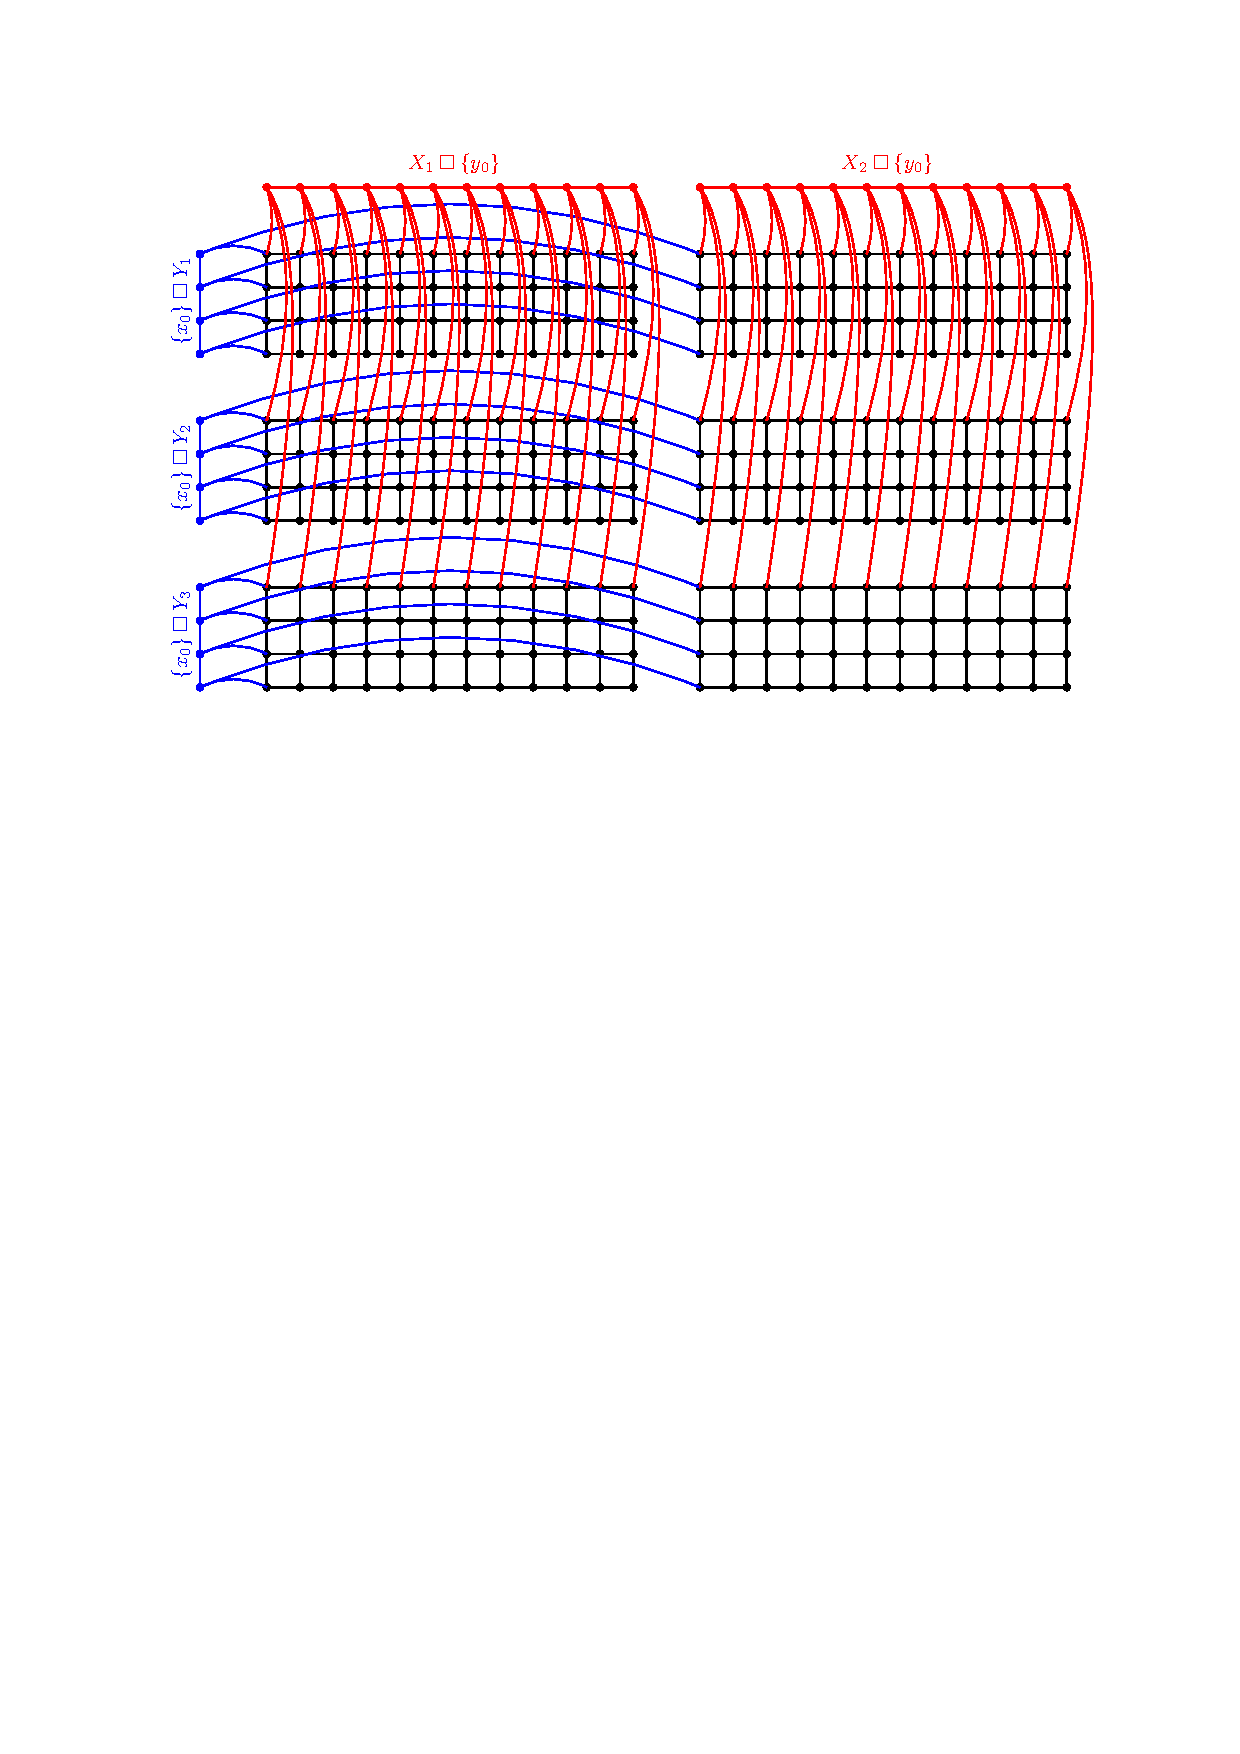
\includegraphics{t1xt2}
    \end{center}
    \caption{The graph $S_{2,12}\boxprod S_{3,4}$ is made up of $6$ vertex-disjoint $12\times 4$ grids $G_{1,1},\ldots,G_{2,3}$ joined by $2$ (horizontal) paths, each of size $12$ and $3$ (vertical) paths, each of size $4$.  (The vertex $(x_0,y_0)$ is ommitted from this drawing.)}
    \label{t1xt2}
  \end{figure}

  Let $p_0$ be a fixed positive integer whose value is discussed below. If $p \le p_0$, then $\ell_2 p_0 \ge \ell_2 p_2 \ge N$, so $\ell_2\ge N/p_0$.  In this case $S_{\ell_2,p_2}$ contains a subgraph isomorphic to $S_{\ceil{N/p_0}}$.  By \cref{anything_times_star}, $K_{\ceil{N/p_0}}\preceq S_{\ell_1,p_1}\boxprod S_{\ceil{N/p_0}} \preceq S_{\ell_1,p_1}\boxprod S_{\ell_2,p_2}$.  Since $\gm(K_{\ceil{N/p_0}}) = \floor{\sqrt{N/p_0}}$, this implies that $\gm(S_{\ell_1,p_1}\boxprod S_{\ell_2,p_2}) \ge \floor{\sqrt{N/p_0}}\ge \floor{\sqrt{pN}/p_0}=\Omega(\sqrt{pN})$.  Therefore, we may assume that $p\ge p_0$.

  TODO: Using the lower bound on $p$, explain how to reduce the values of $\ell_i$ and $p_i$ by constant factors so that
   \begin{compactenum}
     \item $p$ is even;
     \item $p_1 = 3ap$ for some positive integer $a$;
     \item $\ell_1p_1 = 4N$ and $\ell_2 p=5N$; and
     \item $N/p$ is a perfect square
   \end{compactenum}
   % By reducing $p_1$ by a factor of at most two, we may assume that $p$ divides $p_1$, so $p_1=ap$ for some integer $a\ge 1$.  If $k_2 < a$ then we may discard paths in $\PP_1$ to reduce their number to $k_2$ and shorten each path in $\PP_1$ so that they all have $p_2$ vertices.  This does not change $N$ or $p$.  If $k_2 \ge a$ then we can discard $k_2\bmod a$ paths from $\PP_2$ so that $k_2$ becomes a multiple of $a$.  This reduces $k_2$ by a factor of at most two.  Finally, we can remove paths from $\PP_1$ so that $p_1k_1 = apk_1 = pk_2$.  This does not decrease $p$ or $N$.  Therefore, we may assume that $\PP_1:=\{P_{1,1},\ldots,P_{1,k}\}$ contains $k$ paths, each of having $ap$ vertices and $\PP_2:=\{P_{2,1},\ldots,P_{2,ak}\}$ contains $ak$ paths, each having $p$ vertices.  In this way, $N=apk$.


  Our plan is to piece together $N/p$ disjoint models of $\boxplus_{p/2}$ in order to obtain a model of a grid with side length $\tfrac{p}{2}\sqrt{N/p}=\tfrac{1}{2}\sqrt{pN}$.  Refer to \cref{subgrid}.  Observe that, within $S_{\ell_1,p_1}\boxprod S_{\ell_2,p_2}$, each vertex in the first row of $G_{i,j}$ is adjacent to a distinct vertex in $X_i\times\{y_0\}$. It is helpful to think of $X_i\times\{y_0\}$ as a hidden zeroth row of $G_{i,j}$ and note that this row is shared among $G_{i,j'}$ for all $j\in[\ell_2]$.  We use the notation $G_{i,j}^+$ to denote the subgraph of $S_{\ell_1,p_1}\boxprod S_{\ell_2,p_2}$ induced by $V(G_{i,j})\cup (X_i\times\{y_0\})$

  As illustrated in \cref{subgrid}, $G_{i,j}^+$ contains a model of $\boxplus_{p/2}$ in which each of the four degree-$2$ vertices of $\boxplus_{p/2}$ has a branch set that contains two distinct vertex of $X_i\times\{y_0\}$ and each of the $2p-4$ degree-$3$ vertices of $\boxplus_{p/2}$ has a branch set that contains one distinct vertex in $X_i\times\{y_0\}$.  In all, these branch sets contain exactly $2p$ vertices, $\{x_{i,s},x_{i,s+1},\ldots,x_{i,s+2p-1}\}\times\{y_0\}$, of the path $X_i\boxprod\{y_0\}$. We call this model is the \defn{canonical model} of $\boxplus_{p/2}$ in $G_{i,j}^+$ that \defn{starts} at $x_{i,s}$.

  \begin{figure}
    \begin{center}
      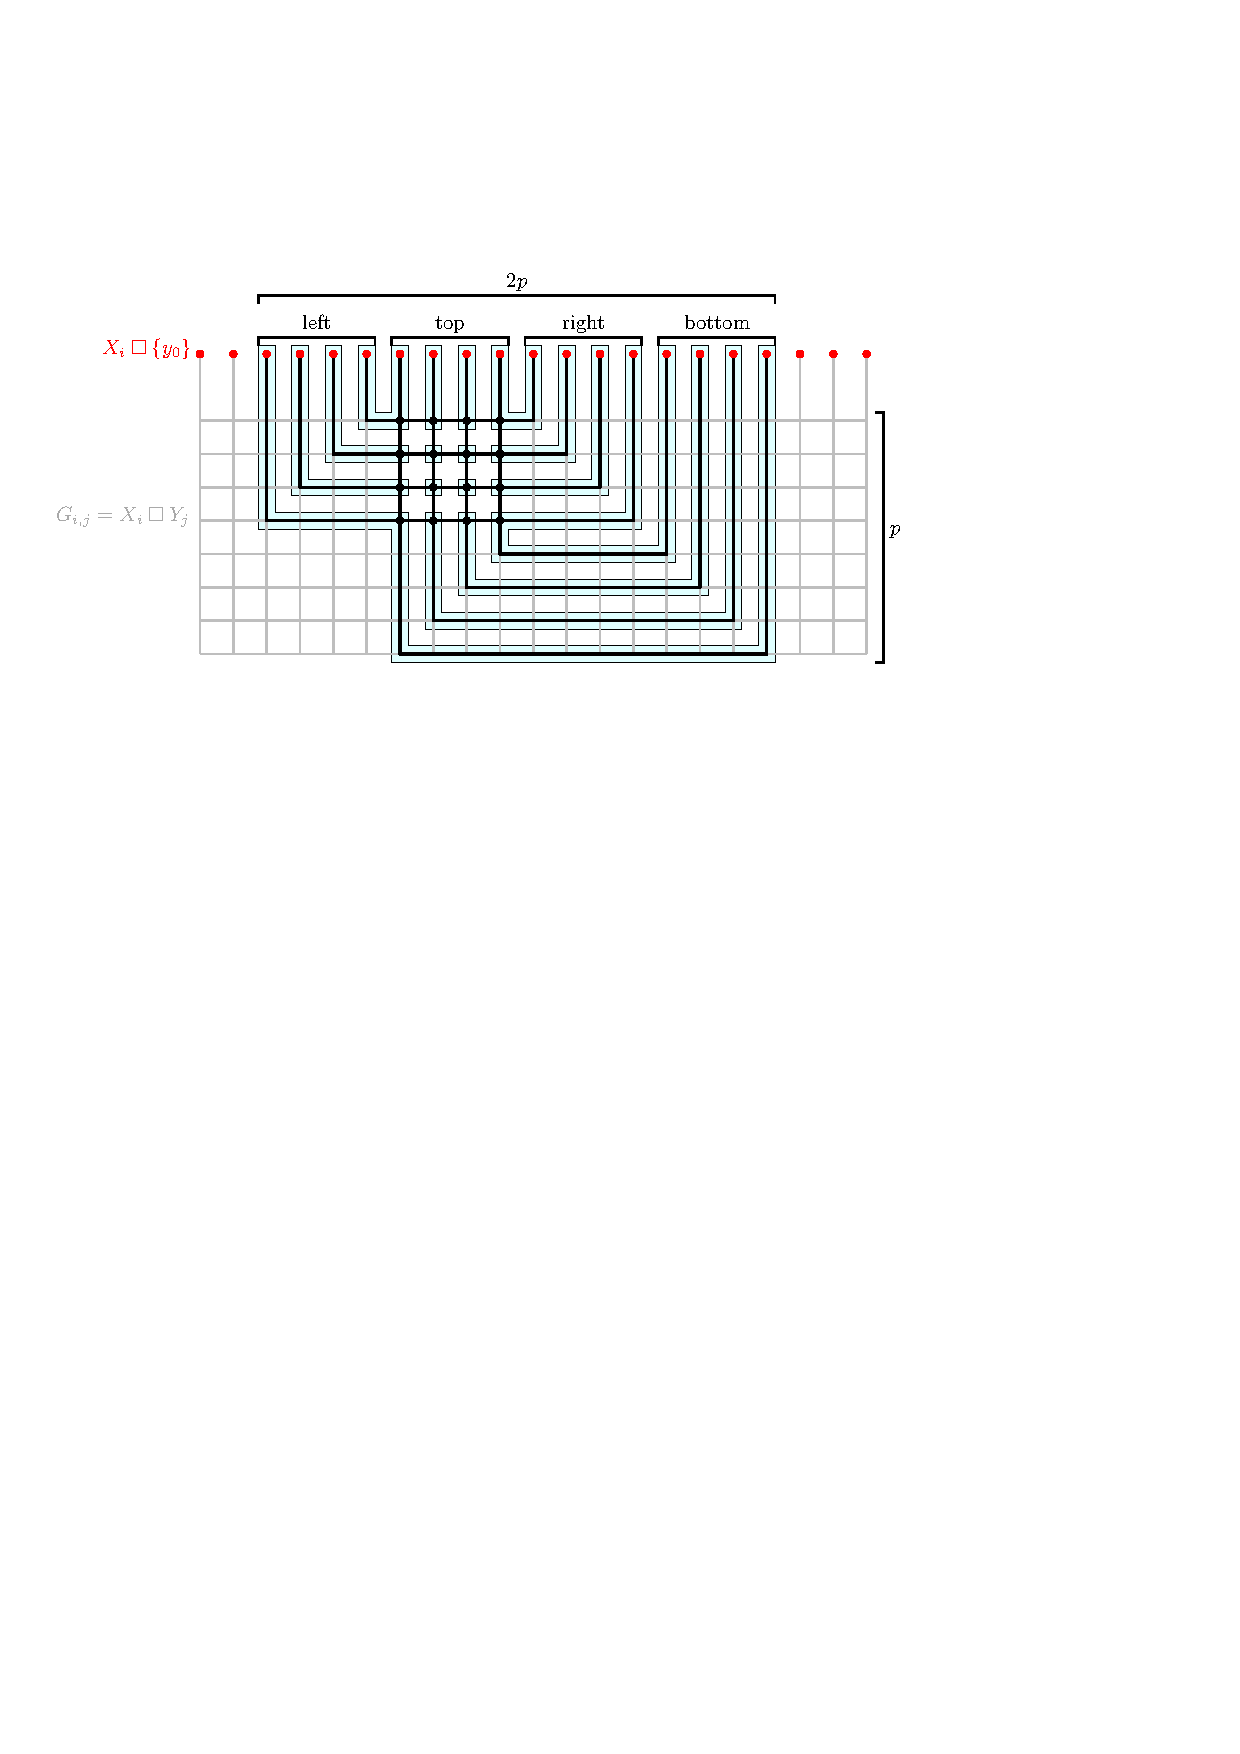
\includegraphics{subgrid}
    \end{center}
    \caption{One of the $\tfrac p2\times \tfrac p2$ subgrids used in the proof of Lemma~\ref{star_times_star}, which is contained in one of the $2ap\times p$ grids contained in $S_{\ell_1,p_1}\boxprod S_{\ell_2,p_2}$.}
    \label{subgrid}
  \end{figure}

  For each $k\in[N/p]$ we let $\mathcal{M}_k$ be the canonical model of $\boxplus_{p/2}$ in $G_{\ceil{k/a},5k}^+$ and that starts at $x_{\ceil{k/3p},1+3p(k\bmod a)}$.  Before continuing, it is worth discussing the choices of parameters that define $\mathcal{M}_k$.  Let $i:=\ceil{k/a}$, let $j:=5k$, and let $s:=1+3p(k\bmod a)$.  We can think of $G_{1,1},\ldots,G_{\ell_1,\ell_2}$ as being organized into an $\ell_1\times \ell_2$ matrix with $\ell_1$ columnns and $\ell_2$ rows, as in \cref{t1xt2}.  In this matrix, rows $j,\ldots,j+4$ are devoted entirely to $\mathcal{M}_{k}$.  On the other hand, each column $i$ of this matrix will contain $a$ models of $\boxplus_{p/2}$.  Each of these models will use some of the $3ap$ vertices in $X_i\boxprod\{y_0\}$.  The choice of starting point $s$ ensures that $3p$ of the vertices in $X_i\boxprod\{y_0\}$ can be used by $\mathcal{M}_k$.

  % We claim that, for any $1\le k_1 < k_2\le N/p$, $\mathcal{M}_{k_1}$ and $\mathcal{M}_{k_2}$ are vertex disjoint, that is $\cup\mathcal{M}_{k_1}\cap\cup\mathcal{M}_{k_2}=\emptyset$. Let $i_b:=\ceil{k_b/a}$ and $j_b:=5k_b$ for each $b\in\{1,2\}$.  Then $\cup\mathcal{M}_{k_b}\subseteq V(G^+{i_b,j_b})$ for each $b\in\{1,2\}$. The subgraphs $G_{i_1,j_1}$ and $G_{i_2,j_2}$ are vertex disjoint, except when $i:=i_1=i_2$, in which case these two graphs both contain all the vertices in $X_i\times\{y_0\}$.
  % However, $\mathcal{M}_{k_1}$ starts at $(x_{i,1+3p(k_1\bmod a)},y_0)$ while $\mathcal{M}_{k_2}$ starts at $(x_{i,1+3p(k_2\bmod a)},y_0)$.  Since $\ceil{k_1/a}=i_1=i_2\ceil{k_2/a}$ and $k_1\neq k_2$, $1 \le |k_1-k_2| < ap$, so $k_1\bmod a\neq k_2\bmod a$.  Therefore $(x_{i,1+3p(k_1\bmod a)},y_0)$ and $(x_{i,1+3p(k_2\bmod a)},y_0)$ are separated by at least $3p$ vertices $X_i\boxprod\{y_0\}$.  Since each of these models uses only $2p$ consecutive vertices of $X_i\boxprod\{y_0\}$, there is no vertex of $X_i\boxprod\{y_0\}$ used in both models.

  In order to merge these $N/p$ vertex disjoint models of $\boxplus_{p/2}$ into a single model of $\boxplus_{\tfrac 12\sqrt{pN}}$, some of the branch sets of each model $\mathcal{M}_k$ will be extended so that they become adjacent the appropriate branch sets in some other models.  In particular, if $\mathcal{M}_k$ has a $\boxplus_{p/2}$ model $\mathcal{M}_{k'}$ to its left, then the $p/2$ branch sets of $\mathcal{M}_k$ corresponding to the left boundary of $\boxplus_{p/2}$ should be extended so that they are adjacent to the $p/2$ branch sets of $\mathcal{M}_{k'}$ corresponding to the right boundary of $\boxplus_{p/2}$.  Similarly, if some $\boxplus_{p/2}$ model $\mathcal{M}_{k''}$ is directly above $\mathcal{M}_k$, then the $p/2$ branch sets of $\mathcal{M}_k$ corresponding to the top of $\boxplus_{p/2}$ should be extended so that they are adjacent to the $p/2$ branch sets of $\mathcal{M}_{k''}$ corresponding to the bottom boundary of $\boxplus_{p/2}$.  We now explain how to do this.

  Let $i:=\ceil{k/a}$, $j:=5k$, and $s:=1+3p(k\bmod a)$. Define $i'$, $j'$, and $s'$ similarly, using $k'$ in place of $k$.  To extend the branch sets from $\mathcal{M}_k$ to $\mathcal{M}_{k'}$ we will make use of vertices in $G_{i,j+1}$, $G_{i,j+2}$ and $G_{i',j+2}$, none of which contains vertices used by $\mathcal{M}_t$ for any $t\in[N/p]$.  It will also make use of an additional $p/2$ vertices of $X_i\boxprod\{y_0\}$.\footnote{The additional vertices of  $X_i\boxprod\{y_0\}$ that are used when extending $\mathcal{M}_k$ is the reason we have chosen $p_1=3ap$ rather than $p_1=2ap$.  We are reserving $3p$ consecutive vertices of $X_{i}\boxprod\{y_0\}$ for $\mathcal{M}_k$.}  There are two cases to consider:
  \begin{compactenum}
    \item $i = i'$.  See Figure~\ref{modeller_i}. In this case, we extend the $p/2$ branch sets corresponding to the left side of $B_k$ through $G_{i,j+1}$ through $G_{i,j+1}$ to the vertices of $X_i\times\{y_0\}$ contained in the $p/2$ branch sets of $B_{k'}$ corresponding to the right side of $B_{k'}$.
  \begin{figure}[htbp]
    \begin{center}
        \includegraphics[page=2]{modeller}
    \end{center}
    \caption{Extending $\mathcal{M}_k$ so that is branch sets meet $\mathcal{M}_{k'}$, case 1.}
    \label{modeller_i}
  \end{figure}

    \item $i\neq i'$.  See Figure~\ref{modeller_ii}.  In this case, we extend the $p/2$ branch sets of $\mathcal{M}_k$ corresponding to the leftmost column of $\boxplus_{p/2}$ through $G_{i,j+1}$ into $(x_{i,s+2p},y_0),\ldots,(x_{i,s+5p/2},y_0)$.  Next we continue to extend these branch sets through $G_{i,j+2}$ to any $p/2$ vertices in $\{x_0\}\times Y_j$. From there, we extend branch sets through $G_{i',j+2}$ to the vertices of $X_{i'}\times\{y_0\}$ contained in the $p/2$ branch sets of corresponding to the right side of $\boxplus_{p/2}$.

    We note that the (superfluous looking) routing through $G_{i,j+1}$ is actually necessary, otherwise the branch set for the top left vertex of $\boxplus_{p/2}$ modelled by $\mathcal{M}_k$ will only become adjacent to the bottom right vertex of $\boxplus_{p/2}$ modelled by $\mathcal{M}_{k'}$.  Indeed, without this step, the adjacencies between the left column of $M_{k}$ and right column of $M_{k'}$ will be completely reversed.
  \begin{figure}[htbp]
    \begin{center}
        \includegraphics[page=3]{modeller}
    \end{center}
    \caption{Extending $\mathcal{M}_k$ so that is branch sets meet $\mathcal{M}_{k'}$, case 2.}
    \label{modeller_ii}
  \end{figure}
  \end{compactenum}
  The extension of the branch sets of $\mathcal{M}_{k}$ to those of $\mathcal{M}_{k''}$ is done the same way, but the routing is done through $G_{i,j+3}$, $G_{i,j+4}$, $G_{i',j+4}$ and the remaining $p/2$ vertices of $X_i\boxprod\{y_0\}$ that are reserved for $\mathcal{M}_k$.

  All that remains is to verify that $\mathcal{M}:=\bigcup_{k=1}^{N/p}\mathcal{M}_k$ is indeed a model of $\boxplus_{\tfrac 12\sqrt{pN}}$.  That each branch set of $\mathcal{M}$ induces a connected subgraph of $S_{\ell_1,p_2}\boxprod S_{\ell_2,p_2}$ is clear from construction.

  Next we verify that, that the branch sets in $\mathcal{M}_{k_1}$ are vertex-disjoint from those in $\mathcal{M}_{k_2}$, for any $k_1\neq k_2$. For each $b\in\{1,2\}$, if $\mathcal{M}_{k_b}$ was originally contained in $G^+_{i_b,j_b}$ then, after extending it, all but at most $3p$ of the vertices used in $\mathcal{M}_{k_b}$ are contained in $Z_{b}:=\bigcup_{i\in[\ell_1]}\bigcup_{c=0}^4 G_{i,j_b+c}$. The remaining (at most $3p$) vertices in $\mathcal{M}_{k_b}$ are taken from $3p$ consecutive vertices of $X_{i_b}\boxprod\{y_0\}$.  The definition of $j_b$ ensures that $|j_1-j_2|\ge 5$, so $Z_{1}\cap Z_2=\emptyset$.  The choice of start vertex $x_{i_b,s_b}$ in $X_{i_b}$ for the canonical model $\mathcal{M}_{k_b}$ ensures that $i_1\neq i_2$ or $|s_1-s_2|\ge 3p$.  In the former case we are done.  In the latter case, $(\cup M_{k_b})\cap (V(X_{k_b})\times\{y_0\})=(x_{i,s_b},y_0),\ldots,(x_{i,s_b+3p-1},y_0)$ so the condition $|s_1-s_2|\ge 3p$ ensures that $\mathcal{M}_{k_1}$ and $\mathcal{M}_{k_2}$ are disjoint.

  Finally, we check that, if $xy\in E(\boxplus_{\tfrac 12\sqrt{pN}})$ then some there is some edge $vw$ of $S_{\ell_1,p_1}\boxprod S_{\ell_2,p_2}$ with $v$ in the branch set $B_x$ of $x$ and $w$ in the branch set $B_y$ of $y$.  If the edge $xy$ has both endpoints in a single $p/2\times p/2$ subgrid, then this is easily verified by the construction of the model $\mathcal{M}_k$ of that subgrid (\cref{subgrid}).  If $v$ and $w$ belong to different subgrids $X$ and $X'$ then, without loss of generality, $X$ is below $X'$ or $X$ is to the right of $X'$.  In this case, the model $\mathcal{M}_{k}$ of $X$ was extended so that the branch sets of the vertices in its top row (respectively, left column) become adjacent to the appropriate branch sets of the model $\mathcal{M}_{k'}$ of $X'$.
\end{proof}

This establishes our lower bound on the largest grid minor contained in a graph product:

\begin{thm}\label{lower_bound}
  If $G_1$ and $G_2$ are connected graphs with $n_1$ and $n_2$ vertices, respectively, and $n:=\min\{n_1,n_2\}$, then $\gm(G_1\boxprod G_1)\in\Omega(\sqrt{n})$
\end{thm}

\begin{proof}
  For each $b\in\{1,2\}$, let $T_b$ be a tree contained in $G_b$ with exactly $n$ vertices.  By Corollary~\ref{subdivided_star_minor_ii}, there exists $\ell_b,p_b$ with $\ell_b p_b^2\in\Omega(n)$ such that $S_{\ell_b,p_b}\preceq T_b$. \pat{We don't immediately get our result from \cref{star_times_star} because $p=\min\{p_1,p_2\}$.  To see this, consider the case where $p_1=1$, $\ell_1=n$, $p_2=\log n$ and $\ell_2=n/\log^2 n$.  Then $p=1$ and $N=p_2\ell_2=n/\log n$ so \cref{star_times_star} only guarantees that $\gm(G_1\boxprod G_2)=\Omega(\sqrt{p N})=\Omega(\sqrt{n/\log n})$.  Of course, \cref{anything_times_star} handles this, but....}

  Right now, the best argument I can think of is to branch on the value of $p$.  Apply \cref{newer_subdivided_star_minor} to each of $G_1$ and $G_2$ and suppose that $p_1< p_2$.  If $p:=p_1 < \sqrt{\log n}$ then use \cref{anything_times_star} to deduce that $G_1\boxprod G_2\succeq K_{n/p}\succeq K_{n/\sqrt{\log n}}\succeq \boxplus_{\sqrt{n}/\log^{1/4} n}$, so $\gm(G_1\boxprod G_2)=\Omega(\sqrt{n}/\log^{1/4} n)$.  Otherwise, apply \cref{new_subdivided_star_minor} to $G_2$ to deduce that $G_2\succeq S_{\ell_2,p_2}$ with $\ell_2p_2 \ge n/\log n$ (and $p_2\ge \log^{1/4} n$?).  Then apply \cref{star_times_star} to deduce that $\gm(G_1\boxprod G_2)=\Omega(\sqrt{p\ell_2p_2}) \ge \sqrt{n/\sqrt{\log n}}=\Omega(n/\log^{1/4} n)$.

  % Let $\ell = \min\{\ell_1, \ell_2\}$ and $p = \min\{p_1, p_2\}$. Then, by Lemma~\ref{star_times_star}, $\gm(S_{\ell_1,p_1}\boxtimes S_{\ell_2,p_2})\in\Omega(\sqrt{pN}) = \Omega(\sqrt{\ell p^2}) = \Omega(\sqrt{n})$. Since $S_{\ell_b,p_b}\preceq T_b\preceq G_b$ for each $b\in\{1,2\}$, the result follows from two applications of Observation~\ref{minor_product}.
\end{proof}

\section{The Upper Bound}

The following construction shows that the lower bound in Theorem~\ref{lower_bound} is optimal.

\begin{lem}\label{upper_bound}
  $\gm(S_n\boxtimes P_n)\le \sqrt{5n}$
\end{lem}

\begin{proof}
  Suppose that $S_n\boxtimes P_n$ contains a $\boxplus_k$ grid minor.  We will prove that $k\le\sqrt{5n}$.  Let $\mathcal{M}:=(B_x:x\in V(\boxplus_k))$ be a model of $\boxplus_k$ in $G$.  We say that a piece $B_x$ of $\mathcal{M}$ is \defn{rooty} if $(x_0,y)\in V(B_x)$ for some $y\in V(P)$ and $B_x$ is \emph{rootless} otherwise.  Clearly, the number of rooty parts in $\mathcal{M}$ is at most $n$.

  Observe that each rootless part $B_x$ of $\mathcal{M}$ is a single path $(x_i,y_j),\ldots,(x_i,y_{j+\ell})$.  There are at most two other rootless parts [one containing $(x_i,y_{j-1})$ and one containing $(x_i,y_{j+\ell+1})$] adjacent to $B_x$.  However, the vertex $x$ has degree at least $3$ in $\boxplus_k$, so $B_x$ must be adjacent to at least one rooty part $B_y$ such that $xy$ is an edge of $\boxplus_k$; we call this a \emph{rooty-rootless adjacency}. The model $\mathcal{M}$ has $k^2$ parts and at most $n$ of these are rooty, so there are at least $k^2-n$ rootless parts.  Therefore, there are at least $k^2-n$ rooty-rootless adjacencies.  Each rooty part of $\mathcal{M}$ can account for at most $4$ of these adjacencies, so $k^2-n \le 4n$, proving the result.\footnote{We could actually prove a bound of $\approx\sqrt{2n}$ by using the fact that most rootless parts need to be adjacent to $2$ rooty parts.}
\end{proof}

\section{Discussion}

% The treewidth of graph products is well understood. For any two connected graphs $G_1$ and $G_2$, $\tw(G_1\boxprod G_2)\in\Theta(n)$.  Therefore, Theorems~\ref{lower_bound} and \ref{upper_bound} give a nearly tight relationship between the largest grid minor and the treewidth of a product:
%
% \begin{cor}\label{treewidth_vs_gm}
%   Let $G_1$ and $G_2$ be any two connected graphs and let $G:=G_1\boxprod G_2$. Then $\gm(G)=\Omega(\sqrt{\tw(G)}/\log \tw(G))$.  Furthermore, there exists two graphs $G_1$ and $G_2$ for which $\gm(G)=O(\sqrt{\tw(G)})$.
% \end{cor}
%
% Corollary~\ref{treewidth_vs_gm} is somewhat unfortunate, for the following reason:  It is know that, for every planar graph $G$, $\gm(G)\in\Theta(\tw(G))$. A weaker version property, the so-called \defn{subquadratic grid minor (SQGM) property} has been used crucially to obtain very efficient approximation algorithms for NP-hard problems on planar graphs and a number of related graph classes.
%
% The product structure theorem for planar graphs has been used to successfully tackle a number of combinatorial problems on planar graphs by using the fact that every planar graph is isomorphic to a subgraph of the strong product of a small treewidth graph $H$ and a path $P$. Indeed, the proofs of these results ignore the original planar graph and are proven directly on the product $H\boxtimes P$.  (The second half of) Corollary~\ref{treewidth_vs_gm} shows that graph products do not necessarily have the SQGM property, so this step loses a property of planar graphs that seems critical in the approximation frameworks mentioned in the preceding paragraph.

Here are some problems I haven't given much thought to.

\begin{compactitem}
  \item Can the techniques in the SQGM approximation framework be adapted to give efficient approximation algorithms for problems on subgraphs of $H\boxtimes P$ where the treewidth $H$ is bounded and $P$ is a path?  These techniques are not immediately applicable to such problems, due to \cref{upper_bound}.

  \item Is it true that for every $n$-vertex planar graph $G$, there exists a bounded treewidth graph $H$ and a path $P$ such that $G$ is isomorphic to a subgraph of $H\boxtimes P$ and, for every $n$-vertex subgraph $G'$ of $H\boxtimes P$, $\tw(G')\in O(\tw(G))$?
\end{compactitem}

{\fontsize{10pt}{11pt}\selectfont
\bibliographystyle{DavidNatbibStyle}
\bibliography{DavidBibliography}}


\appendix

\section{Homely Decompositions and Other Stuff}

Let $S_k:= K_{1,k}$ be the $k$-leaf star.
Let $P_n$ be the $n$-vertex path.


Let $\beta=(B_x:x\in V(T))$ be a $T$-decomposition
of a graph $G$ for some tree $T$. Let  $T_v:=T[\{x\in V(T):v\in B_x\}]$ for each vertex $v$ of $G$. Say $(H_v:v\in V(G))$ is a \defn{home-assignment} if
$H_v\subseteq V(T_v)$ for each $v\in V(G)$;
$H_v\cap H_w=\emptyset$ for all distinct $v,w\in V(G)$; and for each edge $vw\in E(G)$, $w\in B_x$ for some $x\in H_v$, or $v\in B_x$ for some $x\in H_w$. Say $\beta$ is \defn{homely} if it has a home-assignment.

\begin{lem}
\label{Homely}
For any tree $T_1$ with at least $k$ leaves, and for any tree $T_2$, if a graph $G$ has a homely $T_2$-decomposition of width less than $k$, then $G$ is a minor of $T_1 \square T_2$.
\end{lem}

\begin{proof}
Let $y_1,\dots,y_k$ be distinct leaves of $T_1$.
Let $S:=V(T_1)\setminus L$. So $S$ induces a subtree of $T_1$.
Let $(B_x:x\in V(T_2))$ be a homely $T_2$-decomposition of $G$.
Let $(H_v:v\in V(G))$ be the corresponding home-assignment.
For each vertex $v$ of $G$, let $A_v:=\{x\in V(T_2):v\in B_x\}$, which induces a subtree of $T_2$. Let $\col:V(G)\to\{1,\dots,k\}$ be a colouring of $G$ such that $\col(v)\neq\col(w)$ whenever $A_v\cap A_w\neq\emptyset$.

Consider a vertex $v$ of $G$ with $i:=\col(v)$. Let
$Y_v:=\{(a,h):a\in V(S),h\in H_v\}$ and $Z_v:=\{ (y_i, x):x\in A_v\}$. Let $X_v$ be the subgraph of $T_1 \square T_2$ induced by $Y_v\cup Z_v$. We now show that $X_v$ is connected. Let $y'_i$ be the neighbour of $y_i$ in $T_1$. So $y'_i\in S$. Since $T_2[A_v]$ is connected, $Y_v$ induces a connected subgraph of $T_1\square T_2$. Since $T_1[S]$ is connected, for each $h\in H_v$, the set $Z_v$ induces a connected subgraph of $T_1\square T_2$. Moreover, $(y'_i,h)\in Y_v$ is adjacent to $(y_i,h)\in Z_v$. Thus
$X_v$ is connected.

We now show that $X_v\cap X_w=\emptyset$ for distinct vertices $v,w\in V(G)$. We have $Y_v\cap Y_w=\emptyset$ since $H_v\cap H_w=\emptyset$.
We have $Z_v\cap Z_w=\emptyset$ since $A_v\cap A_w=\emptyset$ or $\col(v)\neq\col(w)$.
We have $Y_v\cap Z_w=\emptyset$ and $Z_v\cap Y_w=\emptyset$ since $S\cap \{y_1,\dots,y_k\}=\emptyset$.
Hence  $X_v\cap X_w=\emptyset$.

Consider an edge $vw\in E(G)$. By the definition of home-assignment, without loss of generality, $w\in B_h$ for some $h\in H_v$, implying $h\in A_w$.
Let  $j:=\col(w)$, and let $z$ be the neighbour of $y_j$ in $T_1$, so $z\in S$. Then $(z,h)\in V(X_v)$ is adjacent to $(y_j,h)\in V(X_w)$. Thus $(X_v:v\in V(G))$ is a model of $G$ in $T_1 \square T_2$.
\end{proof}

\begin{lem}
\label{HomelyPathDecomposition}
Every $n$-vertex graph has a homely $P_n$-decomposition of width $\pw(G)$.
\end{lem}

\begin{proof}
Say $P_n=(1,2,\dots,n)$.
It is folklore that $V(G)$ can be enumerated $(v_1,\dots,v_n)$ so that $G$ has a $P_n$-decomposition $(B_1,\dots,B_n)$ with $|B_i|\leq\pw(G)+1$, where $B_i$ is the leftmost bag containing $v_i$ and
$B_i$ is the leftmost bag for no other vertex.
Let $H_{v_i}:=\{i\}$. For any edge $v_iv_j$ with $i<j$, we have
$v_i\in B_j$. So $(H_{v_i}:i\in[n]\}$ is a home-assignment.
\end{proof}

\cref{Homely,HomelyPathDecomposition} imply:

\begin{cor}
\label{TreePath}
For any $n$-vertex graph $G$ with $\pw(G)\leq k$, for any tree $T$ with at least $k+1$ leaves, $G$ is a minor of $T \square P_n$.
\end{cor}

\begin{cor}
\label{StarPath}
Every $n$-vertex graph $G$ is a minor of $S_{k+1} \square P_n$.
\end{cor}

% \begin{lem}
% If $\pw(G) \leq k$ and $|V(G)|=n$ then $G$ is a minor of $S_{k+1} \square P_n$.
% \end{lem}

% \begin{proof}
% Say $P_n=(1,2,\dots,n)$. We may assume $G$ is a $(k+1)$-colourable interval graph, where $I_v =[\ell_v,r_v]$ is the interval for $v$, where
% $\ell_v,r_v\in\{1,\dots,n\}$ and $\ell_v\leqslant r_v$, and $\ell_v\neq\ell_w$ for distinct $v,w\in V(G)$. If $v$ is coloured $i \in \{1,\dots,k+1\}$, then represent $v$ by the subpath $I_v$ of the copy of $P_n$ associated with the $i$-th leaf of $S_{k+1}$, plus vertex $\ell_v$ in the copy of $P_n$ associated with the root of $S_{k+1}$. This defines a model of $G$ in $S_{k+1} \square P_n$.
% \end{proof}

Curiously, this lemma provides a rough characterisation of graphs with pathwidth $k$, since every minor of $S_{k+1} \square P_n$ has pathwidth $O(k)$. Also, note that an analogous proof shows that if $\tw(G) \leqslant k$ and $|V(G)|=n$ then $G$ is a minor of $S_{k+1} \square T$, for some $n$-vertex tree $T$ (and every minor of $S_{k+1}\square T$ has treewidth $O(k)$).

Applying \cref{StarPath} with $G$ being the $k\times k$ grid (which has pathwidth $k$) gives:

\begin{cor}
\label{GridMinorStarPathProduct}
$\gm( S_k \square P_n ) \geq \min\{k-1,\sqrt{n}\}$.
\end{cor}

%These results are generalised as follows. Let $T$ be  a rooted tree. A $T$-decomposition $(B_x:x\in V(T))$ of a graph $G$ is \defn{spread} if for all distinct vertices $v,w\in V(G)$ the subtrees $T_v$ and $T_2$ have distinct roots, where $T_v:=[\{x\in V(T):v\in B_x\}]$.
%For a tree $T$ and graph $G$, a $T$-decomposition $(B_x:x\in V(T))$ of $G$ is \defn{spread} if there is an injection $h:V(G)\to V(T)$ such that $v \in B_{h(v)}$ for each vertex $v$ of $G$.

% \begin{lem}
% \label{DistinctRoots}
% For any tree $T_1$ with at least $k$ leaves, and for any tree $T_2$, if a graph $G$ has a spread $T_2$-decomposition of width $k$, then $G$ is a minor of $T_1 \square T_2$.
% \end{lem}

% \begin{proof}
% Let $y_1,\dots,y_k$ be distinct leaves of $T_1$.
% Let $S:=T_1-L$. So $S$ is a connected subtree of $T_1$.
% Let $(B_x:x\in V(T))$ be a spread $T_2$-decomposition of $G$.
% For each vertex $v$ of $G$, let $T_v:=[\{x\in V(T):v\in B_x\}]$
% and let $r_v$ be the root of $T_v$.
% Fix a $(k+1)$-colouring of $G$, such that if $T_v\cap T_w\neq\emptyset$ then $\col(v)\neq\col(w)$. For each vertex $v$ of $G$, if $i:=\col(v)$ then let $X_v$ be the subgraph of $T_1 \square T_2$ induced by $\{(a,r_v):a\in V(S)\} \cup\{ (y_i, x):x\in V(T_v)\}$. For distinct vertices $v,w\in V(G)$, $X_v\cap X_w=\emptyset$. For each edge $vw\in E(G)$, since $v,w\in B_x$ for some node $x\in V(T)$, in fact $v\in B_{r_w}$ or $w\in B_{r_v}$. Say $v\in B_{r_w}$ and $i:=\col(v)$ and $j:=\col(w)$. Then
% $\{(a,r_v):a\in V(S)\} \cup\{ (y_i, x):x\in V(T_v)\} \in X_v$
% is adjacent to
% $\{(a,r_v):a\in V(S)\} \cup\{ (y_i, x):x\in V(T_v)\} \in X_w$.
% Thus $(X_v:v\in V(G))$ is a model of $G$ in $T_1 \square T_2$.
% % Let $y_1,\dots,y_k$ be distinct leaves of $T_1$.
% % Let $S:=T_1-L$. So $S$ is a connected subtree of $T_1$.
% % Let $(B_x:x\in V(T))$ be a spread $T_2$-decomposition of $G$.
% % Let $h$ be the corresponding injection.
% % Let $T_v:=[\{x\in V(T):v\in B_x\}]$ for each vertex $v$ in $G$.
% % Fix a $(k+1)$-colouring of $G$, such that if $T_v\cap T_w\neq\emptyset$ then $\col(v)\neq\col(w)$. For each vertex $v$ of $G$, if $i:=\col(v)$ then let $X_v$ be the subgraph of $T_1 \square T_2$ induced by $\{(a,h(v)):a\in V(S)\} \cup\{ (y_i, x):x\in V(T_v)\}$. Then $(X_v:v\in V(G))$ is a model of $G$ in $T_1 \square T_2$.
% \end{proof}


% \begin{lem}
% \label{BasicHomelyDecomp}
% For any graph $G$ and for any tree $T$ with at least $|E(G)|$ leaves, $G$ has a homely $T$-decomposition with width $|V(G)|-1$.
% \end{lem}

% \begin{proof}
% Let $B_x:=V(G)$ for each node $x$ of $T$. So $(B_x:x\in V(T))$ is a $T$-decomposition of $G$. So $T_v:=T$ for each vertex $v$ of $G$. Arbitrarily orient each edge $vw$ of $G$. Let $f$ be an injection from $E(G)$ to the set of leaves of $T$. For each vertex $v$ of $G$, let $H_v:=\{ f(uv): uv \in E(G)\}$. So $H_v\cap H_w=\emptyset$ for all distinct $v,w\in V(G)$. For each oriented edge $vw$ of $G$, if $x=f(vw)$ then $x\in H(w)$ and $v\in B_x$. Hence $(B_x:x\in V(T))$ is \defn{homely}.
% \end{proof}

\begin{lem}
\label{BasicHomelyDecomp}
For any graph $G$ and for any tree $T$ with at least $|E(G)|$ vertices, $G$ has a homely $T$-decomposition with width $|V(G)|-1$.
\end{lem}

\begin{proof}
Let $B_x:=V(G)$ for each node $x$ of $T$. So $(B_x:x\in V(T))$ is a $T$-decomposition of $G$, and $T_v:=T$ for each vertex $v$ of $G$. Arbitrarily orient each edge $vw$ of $G$. Let $f$ be an injection from $E(G)$ to $V(T)$. For each vertex $v$ of $G$, let $H_v:=\{ f(\overrightarrow{uv}): u\in N_G^-(v)\}$. So $H_v\cap H_w=\emptyset$ for all distinct $v,w\in V(G)$. For each edge $\overrightarrow{uv}$ of $G$, if $x=f(\overrightarrow{uv})$ then $x\in H_v$ and $u\in B_x$. Hence $(B_x:x\in V(T))$ is \defn{homely}.
\end{proof}

\cref{Homely,BasicHomelyDecomp} imply:

\begin{cor}
\label{HomelyCor}
For any connected graph $G$,
for every tree $T_1$ with at least $|V(G)|$ leaves, and
for every tree $T_2$ with at least $|E(G)|$ vertices,
$G$ is a minor of $T_1 \square T_2$.
\end{cor}

\begin{cor}
\label{HomelyGrid}
For every tree $T_1$ with $\ell_1$ leaves, and
for every tree $T_2$ with $n_2$ vertices,
$$\gm(T_1 \square T_2)\geq \min\{ \ell_1,n_2/2 \}^{1/2}.$$
\end{cor}

% \begin{cor}
% \label{DistinctRootsCor} \david{INVALID}
% For every tree $T_1$ with at least $\ell_1$ leaves, and for every tree $T_2$ with at least $n_2$ vertices,
% $$\gm(T_1\square T_2)\geq \min\{ \ell_1,n_2\}^{1/2}.$$
% \end{cor}

% \begin{proof}
% Let $n:=\min\{\ell_1,n_2\}$. Let $B_x:=V(K_n)$ for each $x\in V(T_2)$. Let $h$ be an arbitrary injection from $V(K_n)$ to $V(T_2)$. This defines a spread $T_2$-decomposition of $K_n$ with width $n-1$. By \cref{DistinctRoots}, $K_n$ is a minor of $T_1 \square T_2$. Thus, the $\sqrt{n}\times \sqrt{n}$ grid is a minor of $T_1 \square T_2$.
% \end{proof}

%What we need...

% \begin{conj}
% \label{DistinctRootsNeeded}
% For every tree $T_1$ with at least $\ell_1$ leaves,
% and for every tree $T_2$ with at least $n_2$ vertices,
% $$\gm(T_1\square T_2)\geq \min\{ \ell_1^{1/2},n_2^{1/3}\}.$$
% \end{conj}

% \begin{proof}
% Let $m:=\min\{ \ell_1^{1/2},n_2^{1/3}\}$.
% So $m^2\leq \ell_1$ and $m^3\leq n_2$.
% Let $G$ be the $m\times m$ grid.
% The result follows from \cref{DistinctRoots} if $G$ has a spread  $T_2$-decomposition of width $\ell_1$.

% The result follows from \cref{Homely} if $G$ has a homely $T_2$-decomposition of width at most $\ell_1$.

% \label{HomelyCorCor}
% For every tree $T_1$ with $\ell_1$ leaves, and
% for every tree $T_2$ with $n_2$ vertices,
% $$\gm(T_1 \square T_2)\geq \min\{ \sqrt{\ell_1},\sqrt{n_2/2}.$$


% SEE NOTES, USE MULTI-NODE HOMES

% If $T_2$ has a $m^2$-vertex path $P$, then $G$ has a spread $P$-decomposition of width $m<\ell_1$. Done

% Note $G$ has tree-depth $4m$ or thereabouts. So $G$ has a spread $T$-decomposition of width $4m$, where $T$ is the complete 4-ary tree of height $\log_2 m$ (I think) with each edge subdivided $\leq 2m$ times.

% \end{proof}


% \begin{thm}
% For all trees $T_1$ and $T_2$,
% $$\tw(T_1\boxtimes T_2) < 2 \gm(T_1\square T_2)^4.$$
% \end{thm}

% \begin{proof}
% Let $n_i:=|V(T_i)|$. Note that $\tw(T_1\boxtimes T_2)< 2 \min\{n_1,n_2\}$. So it suffices to show that
% $\gm(T_1\square T_2)\geq\min\{n_1,n_2\}^{1/4}$.

% Let $d_i$ be the diameter of $T_i$, and let $\ell_i$ be the number of leaves in $T_i$. Thus $n_i\leq d_i \ell_i$. Hence $d_i\geq n_i^{1/2}$ or $\ell_i\geq n_i^{1/2}$.

% Case 1.
% $d_1\geq n_1^{1/2}$ and $d_2\geq n_2^{1/2}$:
% Then $T_1\square T_2$ contains a $d_1\times d_2$ grid as a subgraph, and
% $$\gm(T_1\square T_2)\geq \min\{d_1,d_2\} \geq \min\{n_1^{1/2},n_2^{1/2}\}=\min\{n_1,n_2\}^{1/2}.$$

% Case 2.
% $d_1\geq n_1^{1/2}$ and $\ell_2\geq n_2^{1/2}$:
% By \cref{GridMinorStarPathProduct},
% $$\gm(T_1\square T_2) \geq \min\{\ell_2-1,d_1^{1/2}\} \geq \min\{n_1,n_2\}^{1/4}.$$

% Case 3.
% $\ell_1\geq n_1^{1/2}$ and $d_2\geq n_2^{1/2}$:
% By \cref{GridMinorStarPathProduct},
% $$\gm(T_1\square T_2) \geq \min\{\ell_1-1,d_2^{1/2}\}  \geq \min\{n_1,n_2\}^{1/4} .$$

% Case 4.
% $\ell_1\geq n_1^{1/2}$ and $\ell_2\geq n_2^{1/2}$:
% Thus $T_i$ contains a star with at least $n_i^{1/2}$ leaves as a minor.
% Hence $T_1\square T_2$  contains $K_{m,m}$ as  minor, where $m\geq\min\{n_1,n_2\}^{1/2}$. Note that $K_{m,m}$ contains a $\ceil{\sqrt{m}}\times \ceil{\sqrt{m}}$ grid as a subgraph.
% Therefore
% $$\gm(T_1\square T_2) \geq \min\{n_1,n_2\}^{1/4}.$$
% \end{proof}

\begin{thm}
For all trees $T_1$ and $T_2$,
$$\tw(T_1\boxtimes T_2) < 2^{5/2} \gm(T_1\square T_2)^3.$$
\end{thm}

\begin{proof}
Let $n_i:=|V(T_i)|$. Note that $\tw(T_1\boxtimes T_2)< 2 \min\{n_1,n_2\}$. So it suffices to show that
$\min\{n_1,n_2\} \leq 2^{3/2} \gm(T_1\square T_2)^3$;
that is,
$\gm(T_1\square T_2)\geq 2^{-1/2} \min\{n_1,n_2\}^{1/3}$.
Let $d_i$ be the diameter of $T_i$, and let $\ell_i$ be the number of leaves in $T_i$. Thus $n_i\leq d_i \ell_i$.

%Case 1.
First suppose that
$d_1\geq n_1^{1/3}$ and $d_2\geq n_2^{1/3}$:
Then $T_1\square T_2$ contains a $d_1\times d_2$ grid as a subgraph, and $$\gm(T_1\square T_2)\geq \min\{d_1,d_2\} \geq \min\{n_1^{1/3},n_2^{1/3}\}=\min\{n_1,n_2\}^{1/3}
> 2^{-1/2} \min\{n_1,n_2\}^{1/3}.$$

% Case 2.
% $d_1\geq n_1^{2/3}$ and $d_2\leq n_2^{1/3}$:
% Thus $\ell_2\geq n_2^{1/3}$:
% By \cref{GridMinorStarPathProduct},
% $$\gm(T_1\square T_2) \geq \min\{\ell_2-1,d_1^{1/2}\} \geq \min\{n_1,n_2\}^{1/3}.$$ (IGNORE -1 FOR NOW)

% Case 3.
% $d_2\geq n_2^{2/3}$ and $d_1\leq n_1^{1/3}$:
% Thus $\ell_1\geq n_1^{2/3}$:
% By \cref{GridMinorStarPathProduct},
% $$\gm(T_1\square T_2) \geq \min\{\ell_1-1,d_2^{1/2}\} \geq \min\{n_1,n_2\}^{1/3}.$$ (IGNORE -1 FOR NOW)

% Case 4.
% $d_1\leq n_1^{1/3}$ and $d_2\leq n_2^{2/3}$:
% Thus $\ell_1\geq n_1^{2/3}$ and $\ell_2\geq n_2^{2/3}$, and each $T_i$ contains a star with at least $n_i^{2/3}$ leaves as a minor.
% Hence $T_1\square T_2$  contains $K_{m,m}$ as  minor, where $m\geq\min\{n_1,n_2\}^{2/3}$. Note that $K_{m,m}$ contains a $\floor{\sqrt{2m}}\times \floor{\sqrt{2m}}$ grid as a subgraph.
% Therefore
% $$\gm(T_1\square T_2) \geq \floor{\sqrt{m}} \geq \min\{n_1,n_2\}^{1/3}.$$

Without loss of generality, now assume that $d_1\leq n_1^{1/3}$.
Thus $\ell_1\geq n_1^{2/3}$.
By \cref{HomelyGrid},
$$\gm(T_1\square T_2)\geq \min\{ \ell_1,n_2/2\}^{1/2}
\geq 2^{-1/2}\min\{n_1,n_2\}^{1/3}.$$

% need $(n_2/2)^{1/2} \geq x n_2^{1/3}$\\
% need $(1/2)^{1/2} \geq x \\

% need $(n_2/2)^{1/2} \geq \frac23 n_2^{1/3}$\\
% need $3(n_2/2)^{1/2} \geq 2 n_2^{1/3}$\\
% need $27 (n_2/2)^{3/2} \geq 8 n_2$\\
% need $(27)^2 (n_2/2)^{3} \geq 8^2 n_2^2$\\
% need $(27)^2 n_2 /8 \geq 8^2 $\\
% need $(27)^2 n_2 \geq 8^3 $\\
% true

% Case 5. $d_1\leq n_1^{1/3}$. Thus $\ell_1\geq n_1^{2/3}$. By \cref{HomelyGrid},
% $$\gm(T_1\square T_2)\geq \min\{ \ell_1,n_2/2\}^{1/2} \geq \min\{n_1,n_2\}^{1/3}.$$

% Case 6. $d_2\leq n_2^{1/3}$. Thus $\ell_2\geq n_2^{2/3}$. By \cref{HomelyGrid},
% $$\gm(T_1\square T_2)\geq \min\{ \ell_2,n_1/2\}^{1/2} \geq \min\{n_1,n_2\}^{1/3}.$$
% \begin{tabular}{l|l|l|l}
% \hline
%               & $d_2$ small & $d_2$ medium & $d_2$ big \\\hline
% $d_1$ small  & 5  / 6     & 5 &  5\\
% $d_1$ medium  & 6         & 1 & 1\\
% $d_1$ large  &  6       & 1 & 1 \\
% \hline
% \end{tabular}
\end{proof}

\david{Can this theorem be improved to:
$$\tw(T_1\boxtimes T_2) < c \gm(T_1\square T_2)^2 \polylog(\gm(T_1\square T_2)).$$}

\david{Is there a corresponding lower bound?
That is, are there families of trees $T_1$ and $T_2$ such that
$$\tw(T_1\boxtimes T_2) \geq  c \gm(T_1\square T_2)^2 \polylog(\gm(T_1\square T_2)).$$
My first guess is to have $T_1=T_2=$ the complete binary tree of height $k$ with each edge at depth $i$ subdivided $2^{k-i}$ times.
}

\pat{Yes, $G:=S_n\boxtimes P_n$ has $\tw(G)=\Theta(n)$ and $\gm(G)=\Theta(\sqrt{n})$}

\david{By my question, I meant: does there exist $c_1,c_2>0$ and families of trees $T_1$ and $T_2$ such that
$$\tw(T_1\boxtimes T_2) \geq  c_1 \gm(T_1\square T_2)^2 \log(\gm(T_1\square T_2))^{c_2}?$$
}





\end{document}
{\fontsize{10pt}{11pt}\selectfont
\bibliographystyle{DavidNatbibStyle}
\bibliography{DavidBibliography}}

%%%%%%%%%%%%%%%%%%%%%
\section{\Large Background}
\label{Background}

We consider simple, finite, undirected graphs~$G$ with vertex-set~${V(G)}$ and edge-set~${E(G)}$. A \defn{clique} in a graph is a set of pairwise adjacent vertices. A graph $G$ is \defn{contained} in a graph $X$ if $G$ is isomorphic to a subgraph of $X$. See \citep{Diestel5} for graph-theoretic definitions not given here.

%Let~${\NN \coloneqq \{1,2,\dots\}}$ and~${\NN_0 \coloneqq \{0,1,\dots\}}$.

For $m,n \in \mathbb{Z}$ with $m \leq n$, let $[m,n]:=\{m,m+1,\dots,n\}$ and $[n]:=[1,n]$.

For graphs $F$ and $G$, an \defn{$F$-decomposition} of $G$ is a collection $(B_x :x\in V(F))$ of subsets of $V(G)$ (called \defn{bags}) indexed by the vertices of $F$, such that (a) for every edge $uv\in E(G)$, some bag $B_x$ contains both $u$ and $v$, and (b) for every vertex $v\in V(G)$, the set $\{x\in V(F):v\in B_x\}$ induces a non-empty connected subgraph of $F$. The \defn{adhesion} of $(B_x:x\in V(F))$ is $\max\{B_x\cap B_y \colon xy\in E(F)\}$. The \defn{width} of $(B_x:x\in V(F))$ is $\max\{B_x \colon x\in V(F)\}-1$. The \defn{torso} of a bag $B_x$ (with respect to $(B_x:x\in V(F))$), denoted by \defn{$\torso{G}{B_x}$}, is the graph obtained from the induced subgraph $G[B_x]$ by adding edges so that $B_x\cap B_y$ is a clique for each edge $xy\in E(F)$.

A \defn{tree-decomposition} is a $T$-decomposition for any tree $T$. The \defn{treewidth} of a graph $G$, denoted by \defn{$\tw(G)$}, is the minimum width of a tree-decomposition of $G$. We say $(B_x:x\in V(T))$ is \defn{rooted} if $T$ is rooted. Then, for each $x\in V(T)$, a clique $C$ in the torso $\torso{G}{B_x}$ is a \defn{child-adhesion clique} if there is a child $y$ of $x$ such that $C\subseteq B_x\cap B_y$.

A graph $H$ is a \defn{minor} of a graph $G$ if $H$ is isomorphic to a graph that can be obtained from a subgraph of $G$ by contracting edges. A graph~$G$ is \defn{$H$-minor-free} if~$H$ is not a minor of~$G$. The graph minor structure theorem of \citet{RS-XVI} shows that $K_t$-minor-free graphs has a tree-decomposition where each torso can be constructed using three ingredients: graphs on surfaces, vortices, and apex vertices. To describe this formally, we need the following definitions.

The \defn{Euler genus} of a surface with~$h$ handles and~$c$ cross-caps is~${2h+c}$. The \defn{Euler genus} of a graph~$G$ is the minimum integer $g\geq 0$ such that there is an embedding of~$G$ in a surface of Euler genus~$g$; see \cite{MoharThom} for more about graph embeddings in surfaces.

Let $G_0$ be a graph embedded in a surface $\Sigma$. Let $F$ be a facial cycle of $G_0$ (thought of as a subgraph of $G_0$). An \defn{$F$-vortex} is an $F$-decomposition $(B_x:x\in V(F))$ of a graph $H$ such that $V(G_0\cap H)=V(F)$ and $x\in B_x$ for each $x\in V(F)$. For $g,p,a\geq0$ and $k\geq1$, a graph $G$ is \defn{$(g,p,k,a)$-almost-embeddable} if for some set $A\subseteq V(G)$ with $|A|\leq a$, there are graphs $G_0,G_1,\dots,G_s$ for some $s\in\{0,\dots,p\}$ such that:
\begin{itemize}
	\item $G-A = G_{0} \cup G_{1} \cup \cdots \cup G_s$,
	\item $G_{1}, \dots, G_s$ are pairwise vertex-disjoint,
	\item $G_{0}$ is embedded in a surface of Euler genus at most $g$,
	\item there are $s$ pairwise vertex-disjoint facial cycles $F_1,\dots,F_s$ of $G_0$, and
	\item for $i\in\{1,\dots,s\}$, there is an $F_i$-vortex $(B_x:x\in V(F_i))$ of $G_i$ of width at most $k$.
\end{itemize}
The vertices in $A$ are called \defn{apex} vertices---they can be adjacent to any vertex in $G$. A graph is \defn{$k$-almost-embeddable} if it is $(k,k,k,k)$-almost-embeddable.

We use the following version of the graph minor structure theorem, which is implied by a result of \citet[Theorem~4]{DKMW12}.

\begin{thm}[\citep{DKMW12}]
\label{GMSTimproved}
For every integer $t\geq 1$ there exists an integer $k\geq 1$ such that every $K_t$-minor-free graph $G$ has a rooted tree decomposition $(B_x\colon x\in V(T))$ such that for every node $x\in V(T)$, the torso $\torso{G}{B_x}$ is $k$-almost-embeddable and if $A_x$ is the apex-set of $\torso{G}{B_x}$, then for every child-adhesion clique $C$ of $\torso{G}{B_x}$, either $C\setminus A_x$ is contained in a bag of a vortex of $\torso{G}{B_x}$, or $|C\setminus A_x|\leq 3$.
\end{thm}

% \pat{There is some ambiguity in the statement of \cref{GMSTimproved}.  The child-adhesion cliques of $\torso{G}{B_x}$ are well-defined, but what exactly are the child-adhesion cliques of $\torso{G}{B_x}-A$?  Where does a child-adhesion clique that contains vertices in $A$ and vertices not in $A$ fit in?  Does the theorem tell us that
% \begin{enumerate}[(i)]
%   \item such child-adhesion cliques don't exist;
%   \item such child-adhesion cliques have size at most $3$; or
%   \item there is no restriction on such child-adhesion cliques (maybe they are not contained in any vortex bag, maybe they contain vertices from more than one vortex, or maybe they're not even restricted to vortices).
% \end{enumerate}}  \david{good point, okay now?}

%\robert{I don't think there is any ambiguity with this theorem because of how child-adhesion clique is defined. The definition given is the following: `for each $x\in V(T)$, a clique $C$ in the torso $\torso{G}{B_x}$ is a \defn{child-adhesion clique} if there is a child $y$ of $x$ such that $C\subseteq B_y$.' I believe you are understanding a child adhesion clique to be equal to $B_y\cap B_x$ but our definition allows $C$ to be a subset of $B_x\cap B_y$. I've slightly adjusted the definition of child adhesion clique so that it is explicit that $C\subseteq B_x\cap B_y$.  }

%\david{The child-adhesion cliques of $\torso{G}{B_x}$ are well-defined with respect to the given $k$-almost embeddable representation of $\torso{G}{B_x}$. But Pat's point (I believe) is that  there is no given $k$-almost embeddable representation of $\torso{G}{B_x}-A_x$, so the child-adhesion cliques of $\torso{G}{B_x}-A_x$ are not well-defined. It is a picky point, but still reasonable. The issue is more important later in the paper where we say ``every child-adhesion clique in $\torso{G}{B_x}-S_x$'' since there is no reason to assume that $\torso{G}{B_x}-S_x$ is $k$-almost embeddable. The key question is what version of \cref{GMSTimproved} is least likely to be misunderstood by our readers? The answer (I think) is the revised version in my comment above. Also, the current version of \cref{GMSTimproved}  does not define $A_x$.}

%\robert{With regards to `there is no reason to assume that $\torso{G}{B_x}-S_x$ is $k$-almost embeddable,' isn't $k$-almost embeddable closed under subgraphs? \david{no} Looking into our later usage of child-adhesion clique, it isn't clear to me what the issue is. The only potential ambiguity I see would be fixed if we instead define a child adhesion clique as follows: `for each $x\in V(T)$, a clique $C$ in the torso $\torso{G}{B_x}$ is a \defn{child-adhesion clique} \emph{of $\torso{G}{B_x}$} if there is a child $y$ of $x$ such that $C\subseteq B_y$' and then add \emph{of $\torso{G}{B_x}$} to each of our usages of it.}

%\david{This does not fix the problem of writing ``of child-adhesion-clique of $\torso{G}{B_x}-S_x$'', which we do later. As I said, the key question is what version of \cref{GMSTimproved} is least likely to be misunderstood by our readers? }

The \defn{strong product} of graphs~$A$ and~$B$, denoted by~${A \boxtimes B}$, is the graph with vertex-set~${V(A) \times V(B)}$, where distinct vertices ${(v,x),(w,y) \in V(A) \times V(B)}$ are adjacent if
	${v=w}$ and ${xy \in E(B)}$, or
	${x=y}$ and ${vw \in E(A)}$, or
	${vw \in E(A)}$ and~${xy \in E(B)}$.

Let $G$ be a graph. A \defn{partition} of $G$ is a set $\PP$ of sets of vertices in $G$ such that each vertex of $G$ is in exactly one element of $\PP$. Each element of $\PP$ is called a \defn{part}. The \defn{width} of $\PP$ is the maximum number of vertices in a part. The \defn{quotient} of $\PP$ (with respect to $G$) is the graph, denoted by \defn{$G/\PP$}, with vertex set $\PP$ where distinct parts $A,B\in \PP$ are adjacent in $G/\PP$ if and only if some vertex in $A$ is adjacent in $G$ to some vertex in $B$. An \defn{$H$-partition} of $G$ is a partition $\PP$ of $G$ such that $G/\PP$ is contained in $H$. The following observation connects partitions to products.

\begin{obs}[\citep{DJMMUW20}]
\label{ObsPartitionProduct}
For all graphs $G$ and $H$ and any integer $p\geq 1$, $G$ is contained in $H\boxtimes K_p$ if and only if $G$ has an $H$-partition with width at most $p$.
\end{obs}

A \defn{layering} of a graph $G$ is a partition $\PP$ of $G$, whose parts are ordered $\PP=(V_0,V_1,\dots)$ such that for each edge $vw\in E(G)$, if $v\in V_i$ and $w\in V_j$ then $|i-j|\leq 1$. Equivalently, a layering is a $P$-partition for some path $P$. Consider a connected graph $G$. Let $r\in V(G)$ and let $V_i:=\{v\in V(G):\dist_G(v,r)=i\}$ for each $i\geq 0$.
Then $(V_0,V_1,\dots)$ is a \defn{\textsc{bfs}-layering} of $G$ rooted at $r$. Let $T$ be a spanning tree of $G$, where for each non-root vertex $v\in V_i$ there is an edge $vw$ in $T$ for some $w\in V_{i-1}$. Then $T$ is called a \defn{\textsc{bfs}-spanning tree} of $G$.

If $T$ is a tree rooted at a vertex $r$, then a non-empty path $P$ in $T$ is \defn{vertical} if the vertex of $P$ closest to $r$ in $T$ is an end-vertex of $P$.

Many recent results show that certain graphs can be described as subgraphs of the strong product of a graph with bounded treewidth and a path \citep{DJMMUW20,DHHW22,DMW,HW21b,DEMWW22,HJMW,UWY22}. For example, \citet{DHHW22} proved the following result (building on the work of \citet{DJMMUW20}).

\begin{lem}[\citep{DHHW22}]
\label{GenusPartition}
Every connected graph $G$ of Euler genus at most $g$ is contained in $H\boxtimes P \boxtimes K_{\max\{2g,3\}}$ for some planar graph $H$ with treewidth 3, and for some path $P$. In particular, for every rooted spanning tree $T$ of $G$, there is a partition $\PP$ of $G$ such that $G/\PP$ is planar with treewidth at most $3$ and each part of $\PP$ is a subset of the union of at most $\max\{2g,3\}$ vertical paths in $T$.
\end{lem}

\david{I wonder if the cubic power here is tight.
Here is a key example. Let $p$ be any positive integer.
Let $T$ be the tree obtained from the $p^2$-leaf star by subdividing each edge $p$ times.
So $n = p^3$ (roughly) and it is easily seen that $\tw(T \boxtimes T)$ is within a constant factor of $p^3$ (hint: construct the obvious bramble).
Since $T$ has a path on $2p$ vertices, $T\square T$ contains the $p\times p$ grid. The above theorem also shows $\gm(T\square T) \geq 2p$, and in fact, both cases of the proof show that
$\gm(T\square T) \geq \Omega(p)$.
Speculative Conjecture: $\gm(T \square T) \leq O(p)$. \\
This would improve the long-standing best known lower bound on the grid-minor-theorem of Robertson and Seymour.
So I am probably wrong, but it is worth trying to work it out. }

\pat{Unfortunately, it looks like $T\square T$ contains an $\Omega(p^2) \times \Omega(p^2)$ grid minor, so we don't get any better upper bound for the Grid Minor Theorem. The idea is that $T*T$ contains $p^4$ $p\times p$ grids that are glued together along a total of $2p^2$ sides (the top and left side of each grid).  You can think of these as tiles and each one contains a $p/2 \times p/2$ grid model where each part of the model contains a vertex on the top row or left column.  I'm working through the details now just to make sure that it works so we can forget about it.\\
This attached figure is an attempt to give an explanation.  If two squares are in the same column, then their top rows are identified. If two squares are in the same row then their left columns are identified.  Each of the $p^2$ squares on the diagonal will be identified with one $p/2 \times p/2$ subgrid.  The trick then is to include paths in the off-diagonal squares so that sides line up correctly.\\
For example, A shares its left side with the right side of E so the parts of A include (orange) paths an off-diagonal grid to make these parts line up.  \\
There are $p^2$ diagonal squares which is enough for us, and there seems to be tons of room on the off-diagonals to do the routing.
}

%\includegraphics[scale=0.8]{PatConstruction}
